\documentclass[12pt,a4paper]{report}

\usepackage{mathtools}
\usepackage{graphicx}
\usepackage{braket}
\usepackage{amsthm}
\usepackage{amsfonts}
\usepackage{lmodern}
\usepackage[utf8]{inputenc}
\usepackage[french]{babel}
\usepackage[T1]{fontenc}
\usepackage{subcaption}
\usepackage{caption}
\usepackage{gensymb}
\usepackage{tikz}
\usepackage{qcircuit}
\usepackage{listings}
\usepackage{pgfplots}
\usepackage{appendix}
\usepackage{hyperref}
\usepackage[ruled,vlined]{algorithm2e}
\usepackage{titlesec}
\usepackage{cleveref}
\usepackage{float}
\definecolor{gray75}{gray}{0.75}
\DeclareMathOperator{\tr}{tr}
\newcommand{\hsp}{\hspace{20pt}}
\titleformat{\chapter}[display]
{\normalfont%
    \Large% %change this size to your needs for the first line
    \bfseries}{\chaptertitlename\ \thechapter}{15pt}{%
    \Large %change this size to your needs for the second line
    }
\usetikzlibrary{angles,quotes}
% \usepackage{a4wide}

\definecolor{main-color}{rgb}{0.6627, 0.7176, 0.7764}
\definecolor{back-color}{rgb}{0.95,0.95,0.92}
\definecolor{mGreen}{rgb}{0,0.6,0}
\definecolor{string-color}{rgb}{0.3333, 0.5254, 0.345}
\definecolor{key-color}{rgb}{0.8, 0.47, 0.196}

\lstdefinestyle{CStyle}{
  language = C++,
  basicstyle=\tiny,
  backgroundcolor = {\color{back-color}},
  commentstyle=\color{mGreen},
  stringstyle = {\color{string-color}},
  keywordstyle = {\color{key-color}},
  keywordstyle = [2]{\color{blue}},
  keywordstyle = [3]{\color{gray}},
  otherkeywords = {;,<<,>>,++},
  morekeywords = [2]{function,end,Constants,Variables,Minimize,Constraints},
  morekeywords = [3]{tr,EntropyM,EntropyP,EntropyMP,MutualInformation,I,xlog},
  breakatwhitespace=false,
  breaklines=true,
  captionpos=b,
  keepspaces=true,
  numbers=left,
  numbersep=5pt,
  showspaces=false,
  showstringspaces=false,
  showtabs=false,
  tabsize=2,
}


\makeatletter
\newcommand\frontmatter{
    \cleardoublepage
    \pagenumbering{roman}
}
\newcommand\mainmatter{
    \cleardoublepage
    \pagenumbering{arabic}
}
\newcommand\backmatter{
  \if@openright
    \cleardoublepage
  \else
    \clearpage
  \fi
}
\newcommand{\tens}[1]{%
  \mathbin{\mathop{\otimes}\limits_{#1}}%
}

\makeatother
\newcommand{\norm}[1]{\left\lVert#1\right\rVert}
\newcommand{\Mod}[1]{\ (\mathrm{mod}\ #1)}
\graphicspath{{images/}}

\newtheorem{definition}{Définition}
\newtheorem{pb}{Problème}
\newtheorem{rem}{Remarque}
\newtheorem{ex}{Exemple}
\newtheorem{theoreme}{Théorème}

\begin{document}
\begin{titlepage}
    \begin{center}
      \begin{figure}[!tbp]
        \centering
        \begin{subfigure}[b]{0.3\textwidth}
          
\includegraphics[width=\textwidth]{Polytech_Angers.png}
        \end{subfigure}
        \hfill
        \begin{subfigure}[b]{0.3\textwidth}
          
\includegraphics[width=\textwidth]{LogoUnivAngers.png}
        \end{subfigure}
        \hfill
        \begin{subfigure}[b]{0.2\textwidth}
          
\includegraphics[width=\textwidth]{LogoLARIS.png}
        \end{subfigure}
      \end{figure}
      {\large Master Systèmes Dynamiques et Signaux}\\[0.5cm]
      {\large Mémoire de master}\\[0.5cm]
      \rule{\linewidth}{0.5mm} \\[0.4cm]
      { \huge \bfseries Conception de détecteurs quantiques optimaux \\ via le calcul par intervalles \\[0.4cm] }
      \rule{\linewidth}{0.5mm} \\[1.5cm]
      \noindent
      \begin{minipage}{0.4\textwidth}
        \begin{flushleft} \normalsize
          \emph{Auteur :}\\
          M. Pierre \textsc{Engelstein}\\
          \end{flushleft}
          \end{minipage}%
          \begin{minipage}{0.4\textwidth}
          \begin{flushright} \normalsize
          \emph{Encadrants :}\\
          Dr. Nicolas \textsc{Delanoue}\\
          Pr. François \textsc{Chapeau-Blondeau}\\
          \end{flushright}
      \end{minipage}
      \vfill
      \normalsize
      \emph{Jury :}
      \begin{tabular}{lc}
          Pr.~Laurent \textsc{Hardouin}\\
          Dr.~Nicolas \textsc{Delanoue}\\
          Pr.~François \textsc{Chapeau-Blondeau}\\
          Pr.~Sébastien \textsc{Lahaye}\\
          Dr.~Mehdi  \textsc{Lhommeau}\\
          Pr.~David  \textsc{Rousseau}\\
      \end{tabular}

      \vspace{2cm}

      % Version du \\ \today
      % {2020-2021}
    \end{center}
\end{titlepage}

\frontmatter

\section*{Remerciements}
Je remercie Dr. Nicolas Delanoue et Pr. François Chapeau-Blondeau pour leur encadrement sur ce travail. Je remercie également mes parents pour les encouragements et l'aide apportés sur cette année de Master.

\pagebreak
\tableofcontents

\pagebreak
\listoffigures

\mainmatter

\chapter{Introduction}

Lorem ipsum dolor sit amet, consectetur adipiscing elit, sed do eiusmod tempor incididunt ut labore et dolore magna aliqua. Leo vel orci porta non. Tincidunt ornare massa eget egestas purus viverra accumsan in nisl. Tristique senectus et netus et malesuada fames ac turpis egestas. Varius quam quisque id diam vel quam. Rhoncus urna neque viverra justo nec ultrices. Est velit egestas dui id ornare. Arcu non odio euismod lacinia. Ante metus dictum at tempor. Vulputate sapien nec sagittis aliquam malesuada bibendum arcu vitae elementum. Non nisi est sit amet facilisis magna etiam. Quis commodo odio aenean sed adipiscing diam. Etiam erat velit scelerisque in. Tortor id aliquet lectus proin nibh nisl condimentum id. At auctor urna nunc id cursus metus aliquam.

Nec sagittis aliquam malesuada bibendum arcu vitae. Amet nisl purus in mollis. Ac tincidunt vitae semper quis lectus. Ac felis donec et odio pellentesque diam volutpat commodo sed. Ipsum dolor sit amet consectetur adipiscing elit pellentesque. Tortor vitae purus faucibus ornare suspendisse sed nisi. Tristique risus nec feugiat in fermentum posuere urna nec tincidunt. Egestas purus viverra accumsan in nisl nisi scelerisque eu. Ac odio tempor orci dapibus ultrices. Molestie ac feugiat sed lectus vestibulum mattis ullamcorper velit. Interdum velit laoreet id donec ultrices. Donec adipiscing tristique risus nec feugiat in fermentum posuere urna. Porttitor leo a diam sollicitudin. Cras sed felis eget velit aliquet sagittis. Ut etiam sit amet nisl purus in. Viverra suspendisse potenti nullam ac tortor vitae purus faucibus ornare. Lorem ipsum dolor sit amet consectetur adipiscing elit ut aliquam.

\chapter{Informatique quantique: éléments de base}

\section{Postulats de base}

On pose 3 postulats, servant de base aux raisonnements qui suivront. Ces postulats sont des hypothèses de travail, mais confirmés jusqu'a présent par les expériences.

\subsection{Etat d'un système quantique}
Un système quantique peut être représenté par un vecteur d'état, de la même manière qu'un système physique classique. On le représente par la notation de Dirac, notée de la forme $\ket{\psi}$. Ce vecteur d'état est necessairement de norme 1 (la somme des modules au carré vaut 1). On peut distinguer deux types d'états pour un système quantique: les états de base, ou \textbf{états purs}, formant une base vectorielle, et les états superposés. Ces états superposés correspondent à une combinaison linéaire des états purs. On peut écrire généralement un état quantique de la façon suivante:

\begin{equation}
    \ket{\psi} = \displaystyle\sum_{i} c_i \ket{k_i},
\end{equation}

avec les $\ket{k_i}$ états purs, et les $c_i$ respectant $ \displaystyle\sum_{i} |c_i|^2 = 1$ pour la normalité du vecteur d'état.

\medbreak

Dans le cadre de l'informatique quantique, on utilise le système quantique le plus simple, appelé \textbf{qubit}. Ce système quantique est composé de deux états purs, $\ket{0}$ et $\ket{1}$, et des états superposés. Similairement à l'informatique classique, où on travaille sur le système physique le plus élémentaire - le bit - en quantique on travaille sur le système physique quantique élémentaire - le qubit. On dispose des mêmes états purs, mais l'informatique quantique apporte les états \textit{intermédiaires} superposés. Dans la base canonique $\{\ket{0}, \ket{1}\}$, on note un qubit de la façon suivante: $\ket{\psi} = \alpha \cdot \ket{0} + \beta \cdot \ket{1}$.

\subsection{Mesure projective}
Que se passe-t-il quand on mesure un système quantique ? On a évoqué au dessus la notion de superposition des états. L'expérience montre que, lorsqu'on va mesurer un système quantique, on va mesurer au hasard un des états de base, avec comme probabilité le carré du coefficient correspondant.

Mathématiquement, la mesure effectue une projection de l'état du système sur un des états de base dont il est composé. Par exemple, si on a un qubit dans l'état $\ket{\psi} = \frac{1}{\sqrt{2}}\ket{0} + \frac{1}{\sqrt{2}}\ket{1}$, alors la probabilité de mesurer 0, c'est à dire de projeter le système dans l'état pur $\ket{0}$ est $|\frac{1}{\sqrt{2}}|^2 = \frac{1}{2}$; et de même pour l'état pur $\ket{1}$. On a donc exactement la même probabilité de mesurer 0 que de mesurer 1.

Il faut noter que, lorsqu'on fait la mesure, on projete réellement le système quantique dans l'état pur. Concrètement, si on a un état superposé qu'on mesure, il se place dans l'état pur qu'on mesure, et toutes les mesures successives qu'on fera sur ce qubit donneront le même résultat. La mesure fait donc perdre l'état qu'on avait auparavant.

\subsection{Dynamique du système}
Comme n'importe quel système physique, on peut faire évoluer un système quantique dans le temps. Ici apparaissent deux propriétés. Tout d'abord, il découle du premier postulat que la dynamique d'un système quantique est necessairement unitaire. En effet, un système quantique doit, pour être valide, avoir une norme de 1, et donc l'évolution d'un système quantique d'un premier état vers un autre doit conserver cette unitarité. Cela veut dire que la matrice représentant l'évolution du système quantique doit respecter la propriété suivante:

\begin{equation}
    U^{\dagger}U = UU^{\dagger} = I,
\end{equation}

avec $U$ la matrice d'évolution du système, $U^{\dagger}$ la matrice conjuguée transposée de $U$, et $I$ l'identité.

Une deuxième propriété est également posée, ne découlant pas des deux postulats précédents. La dynamique d'un système quantique doit être aussi linéaire. Ainsi, on pourrait penser que n'importe quelle évolution unitaire serait valable, mais l'expérience nous montre que non, il faut en plus qu'elle soit linéaire.

\section{Vers une informatique quantique}
A partir de ces 3 postulats de base, on peut commencer à comprendre comment se construit l'informatique quantique, et quels sont les apports sur l'informatique classique.

\subsection{Multiples qubits}
On a vu la définition d'un qubit. Cela nous permet d'étendre ce système quantique élémentaire à des systèmes composés de multiples qubits. En informatique classique, on travaille quasi systématiquement sur des mots binaires plutôt que des bits uniques; l'équivalent est vrai en quantique. Pour cela, les systèmes quantiques, et donc les qubits, sont munis d'une opération: le produit tensoriel. Quand on veut effectuer une combinaison de deux qubits, cela revient à faire un produit tensoriel des états des deux qubits individuels. Par exemple, si nous disposons de deux qubits ayant pour valeur $\ket{\psi_1} = \ket{0}$ et $\ket{\psi_2} = \ket{1}$, alors on peut écrire le 2-qubit combinaison des deux de la façon suivante:


\begin{equation}
    \ket{\psi} = \ket{0} \tens{} \ket{1},
\end{equation}

qu'on écrit généralement sous la forme plus simple:

\begin{equation}
    \ket{\psi} = \ket{01}.
\end{equation}

Prenons un 2-qubit formé par la combinaison de 2 qubits:

\begin{align*}
\ket{\psi} &= (\alpha_1\cdot\ket{0} + \beta_1\cdot\ket{1}) \otimes (\alpha_2\cdot\ket{0} + \beta_2\cdot\ket{1}) \\
&= \alpha_1\alpha_2 \ket{0} \otimes \ket{0} + \alpha_1\beta_2 \ket{0} \otimes \ket{1} + \beta_1\alpha_2 \ket{1} \otimes \ket{0} + \beta_1\beta_2 \ket{1} \otimes \ket{1} \\
&= \gamma_1 \ket{00} + \gamma_2 \ket{01} + \gamma_3 \ket{10} + \gamma_4 \ket{11}
\end{align*}

On peut donc, si on a un 2-qubit combinaison linéaire de tout les états de bases, le séparer en deux qubits individuels, sur lesquels on va pouvoir agir.

\medbreak

Considérons maintenant le 2-qubit suivant:

\[
\ket{\psi} = \gamma_1 \ket{00} + \gamma_2 \ket{11}
\]

Il parait évident alors qu'on ne peut pas séparer ce 2-qubit en produit tensoriel de 2 qubits individuels. Dans ce cas, on dit que les deux qubits sont \textbf{intriqués} et donc non séparables.


\subsection{Portes quantiques}
Dans la représentation d'état classique, et spécifiquement en informatique, on peut faire évoluer l'état au travers de portes. En informatique classique, on dispose ainsi de portes élémentaires telles que \texttt{AND}, \texttt{NOT}, \texttt{OR}, etc. 

De la même manière, en respectant le troisième postulat posé précédement, on peut construire des portes logiques quantiques, les combiner, afin de créer des circuits quantiques. En informatique quantique, on distingue donc plusieurs portes élémentaires, utilisés dans beaucoup de circuit:

\begin{enumerate}
    \item La porte de Hadamard $H$. Elle permet de passer un qubit d'un état pur $\ket{0}$ à l'état superposé $\frac{1}{\sqrt{2}}\ket{0} + \frac{1}{\sqrt{2}}\ket{1}$, ou de l'état pur $\ket{1}$ à l'état superposé $\frac{1}{\sqrt{2}}\ket{0} - \frac{1}{\sqrt{2}}\ket{1}$. Elle est très utilisée en début de circuit pour préparer les qubits entrants dans un état permettant l'évaluation parallèle de toutes les entrées;
    \item Les portes de Pauli $X$, $Y$ et $Z$ permettant d'effectuer des rotations aux états des qubits;
    \item La porte de Toffoli, équivalent d'un \texttt{NON} booléen, est une porte universelle quantique. Elle permet donc de construire l'ensemble des autres portes faisables.
\end{enumerate}

Un exemple de circuit est le suivant: On dispose d'un 3-qubit dans l'état $\ket{000}$. Au départ, on applique à ces trois qubits une porte de Hadamard, qui les fait se retrouver dans des états équilibrés. On arrive donc à un 3-qubit qui est équilibré entre chacun de ses états purs. On applique ensuite deux portes de Pauli $Z$, un au premier qubit, et un au troisième. Cela est effectivement faisable puisqu'a la sortie des portes de hadamard, les 3 qubits ne sont pas intriqués. On applique de la même façon 3 portes de Hadamard à la sortie, puis on mesure. 

\centerline{
  \Qcircuit @C=1em @R=.7em {
    & \lstick{\ket{0}} & \gate{H} \barrier[-1.25em]{2} & \gate{Z} \barrier[-1.25em]{2} & \gate{H} & \meter & \qwa \\
    & \lstick{\ket{0}} & \gate{H} & \qw & \gate{H} & \meter & \qwa \\
    & \lstick{\ket{0}} & \gate{H} & \gate{Z} & \gate{H} & \meter & \qwa
  }
}

L'avantage du quantique bien montré ici: Les deux portes du milieu vont faire changer l'état des qubits, mais en parallèle: on fait évoluer le système simultanément pour tout les états purs qui nous intéressent, puisqu'ils sont superposés.


% \subsection{Formalisme mathématique}

% \subsubsection*{Qubit unique}

% Le qubit possède deux états de base, correspondant aux états des bits classiques. On les représente par $\ket{0}$, correspondant à l'état $0$ classique, et par $\ket{1}$ pour l'état $1$ classique. A la différence d'un bit classique, un qubit peut également prendre une infinité d'autres états que ses états de base. La question se pose alors de la mesure: que va-t-on mesurer quand un qubit est dans un état autre que $\ket{0}$ ou $\ket{1}$ ? C'est là qu'apparaissent les bizarreries de la mécanique quantique. La mesure va donner au hasard $0$ ou $1$, suivant des probabilités définies.

% Pour représenter ce comportement, on note un qubit de la façon suivante:

% \begin{equation}
% \ket{\psi} = \alpha \cdot \ket{0} + \beta \cdot \ket{1}
% \end{equation}

% Le qubit est alors représenté par une combinaison linéaire des deux états de base $\ket{0}$ et $\ket{1}$, suivant les coefficients complexes $\alpha$ et $\beta$. Ces coefficients représentent les amplitudes de probabilité suivant lesquelles on va mesurer $\ket{0}$ ou $\ket{1}$.

% Ces deux coefficients complexes doivent absolument respecter la propriété suivante:

% \begin{equation}
% \norm{\alpha}^2 + \norm{\beta}^2 = 1
% \end{equation}    

% \subsubsection*{Multiples qubits}

% Une fois ces éléments posés, on peut commencer à travailler avec plusieurs qubits, notés n-qubits. Mathématiquement, une combinaison de qubits correspond à un produit tensoriel de deux vecteurs.

% Prenons les qubits $\ket{0}$ et $\ket{1}$. La combinaisons en un 2-qbits est donc:

% \begin{equation}
%     \ket{\psi} = \ket{0} \tens{} \ket{1}
% \end{equation} 

% qu'on peut écrire plus simplement:

% \begin{equation}
%     \ket{\psi} = \ket{01}
% \end{equation}

% Un 2-qubit a donc 4 états de bases, représentés par: $\{\ket{00},\ket{01}, \ket{10}, \ket{11} \}$, et peut donc être la combinaison linéaire de n'importe quel de ces états de base

% \subsubsection*{Intrication}
% Prenons un 2-qubit formé par la combinaison de 2 qubits:

% \begin{align*}
% \ket{\psi} &= (\alpha_1\cdot\ket{0} + \beta_1\cdot\ket{1}) \otimes (\alpha_2\cdot\ket{0} + \beta_2\cdot\ket{1}) \\
% &= \alpha_1\alpha_2 \ket{0} \otimes \ket{0} + \alpha_1\beta_2 \ket{0} \otimes \ket{1} + \beta_1\alpha_2 \ket{1} \otimes \ket{0} + \beta_1\beta_2 \ket{1} \otimes \ket{1} \\
% &= \gamma_1 \ket{00} + \gamma_2 \ket{01} + \gamma_3 \ket{10} + \gamma_4 \ket{11}
% \end{align*}

% On peut donc, si on a un 2-qubit combinaison linéaire de tout les états de bases, le séparer en deux qubits individuels, sur lesquels on va pouvoir agir.

% \medbreak

% Considérons maintenant le 2-qubit suivant:

% \[
% \ket{\psi} = \gamma_1 \ket{00} + \gamma_2 \ket{11}
% \]

% Il parait évident alors qu'on ne peut pas séparer ce 2-qubit en produit tensoriel de 2 qubits individuels. Dans ce cas, on dit que les deux qubits sont \textbf{intriqués} et donc non séparables.

% \section{Représentation géométrique}

% \section{Programmer un processeur quantique}
\chapter{Calcul par intervalle: éléments de base}

Le calcul par intervalle est décrit au départ dans les travaux de Ramon Moore \cite{Moore66}. L'utilité de ce mode de calcul vient des problèmes que représente le stockage des nombres réels dans nos ordinateurs via la norme \texttt{IEEE 754}. En effet, on sait avec cette norme facilement représenter une certaine quantité, finie de nombres réels tels que $0.5$, sous la forme $\text{signe} \times \text{base}^{exposant} \times (1 + mantisse)$. Il est en revanche impossible de représenter le reste des nombres réels, tels que $0.1$. De ce fait, lorsqu'on se place dans des contextes de calculs, il devient évident qu'on peut se retrouver à accumuler des erreurs de précision qui vont venir fausser les résultats. Quand on veut garantir des résultats, par exemple sur des problèmes d'optimisation, cela peut devenir pénalisant.

\section{Les intervalles}
\subsection{Intervalle et boite}

\begin{definition}
  On définit un \textit{intervalle} $[\underline{x}, \overline{x}]$ comme l'ensemble des nombres réels $x$ tels que $\underline{x} \leq x \leq \overline{x}$.
\end{definition}

On note par la suite plus généralement $[x] = [\underline{x}, \overline{x}]$.

\begin{ex}
  Si on veut représenter le nombre $\sqrt{2} = 1.4142\dots$, on peut dire: $1.4 \leq sqrt(2) \leq 1.5$, donc encadrer ce nombre par l'intervalle $[1.4, 1.5]$.
\end{ex}

\subsection{Fonctions d'inclusion}
% Fonction d'inclusion naturelle
Avec cette notion d'intervalle, on peut définir le comportement quand on applique une fonction. L'idée est de se dire que, pour un intervalle d'entrée $[x]$, l'intervalle image par une fonction $f$ doit contenir l'ensemble des images prises par la fonction $f$ pour tout les $x \in [x]$ :

\begin{definition}
    Soit $f : \mathbb{R}^n \rightarrow \mathbb{R}^m$ une fonction, la fonction $[f] : \mathbb{R}^n \rightarrow \mathbb{R}^m$ est une \textbf{fonction d'inclusion} pour $f$ si

    \begin{align}
        \forall[x] \in \mathbb{R}^n , f([x]) \subset [f]([x])
    \end{align}
\end{definition}

\begin{ex}
  La figure \ref{fig:fct2} montre l'encadrement d'une fonction $y = f(x)$ quelconque. La boite bleue est le produit cartésien de $[x]$ et de $[y]$.

  \begin{figure}[H]
    \centering
    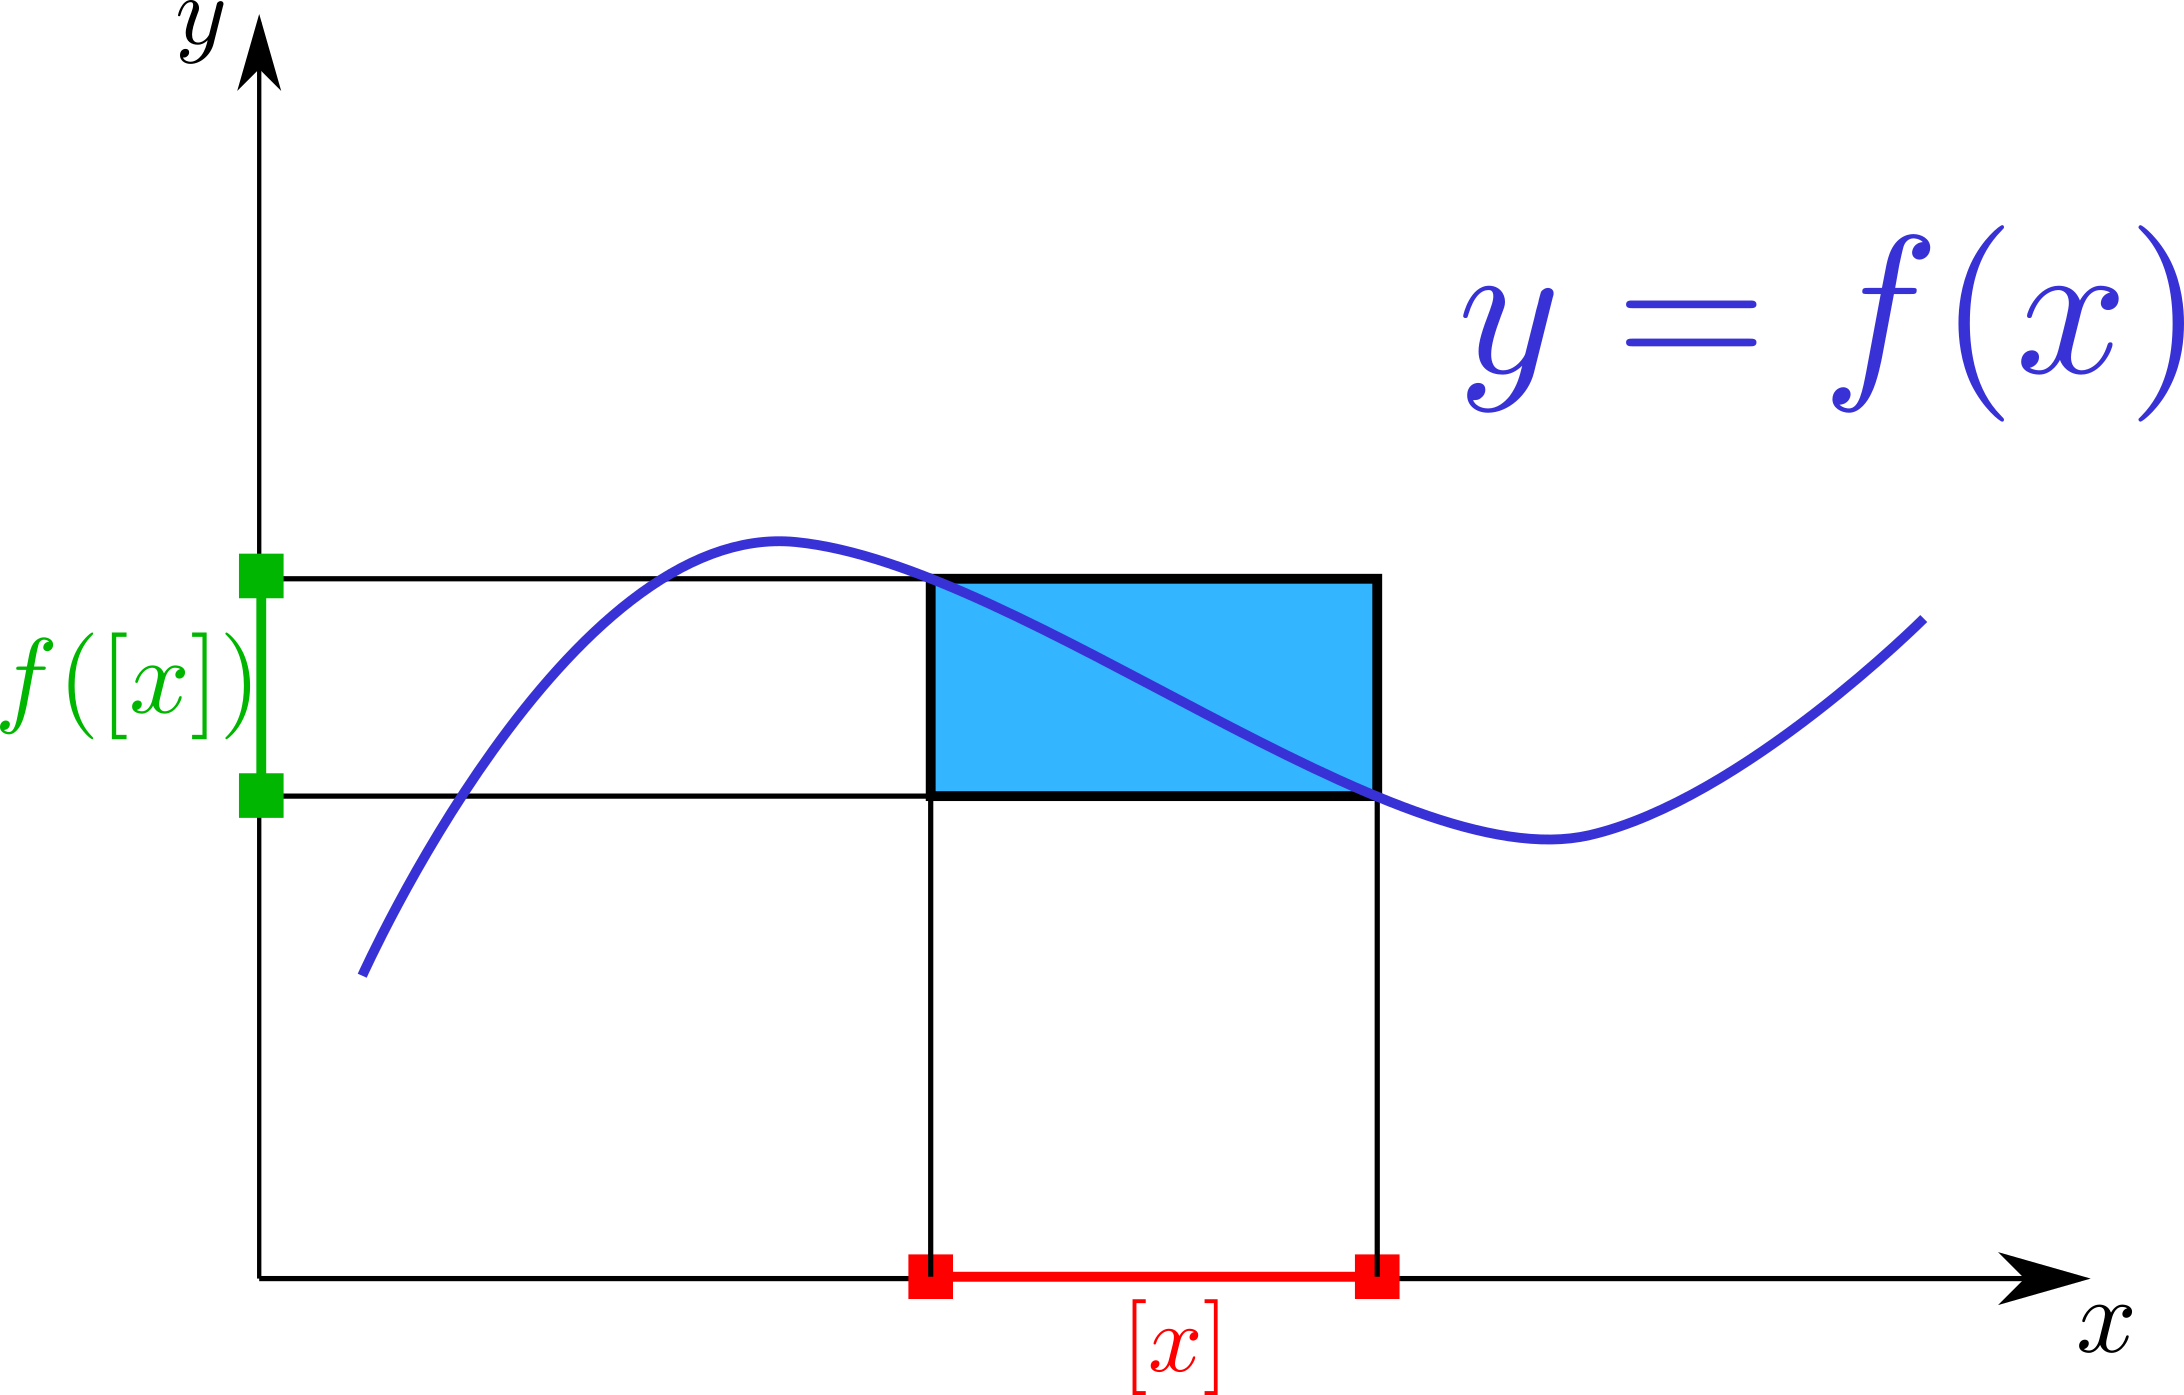
\includegraphics[scale=0.5]{intervaleval/function_eval_2.png}
    \caption{Fonction d'inclusion}
    \label{fig:fct2}
  \end{figure}
\end{ex}

L'encadrement nécessite la connaissance précise de la forme de la fonction pour pouvoir l'encadrer correctement. Ceci peut se révéler compliquer pour des fonctions non évidentes, typiquement quand on monte en dimension. Pour cela, on peut combiner les fonctions d'inclusion sans perdre la garantie d'inclusion, comme indiqué dans le théorème \ref{def:circ}.

\begin{theoreme}
  \label{def:circ}
  si $[f]$ et $[g]$ sont des fonctions d'inclusion respectives pour $f$ et $g$, alors $[f] \circ [g]$ est une fonction d'inclusion pour $f \circ g$.
\end{theoreme}

Cela permet en pratique de construire des fonctions d'inclusions élémentaires puis de les combiner. En effectuant cette opération, on peut en revanche perdre de la précision sur l'encadrement comme le montre la figure \ref{fig:fct3}.

\begin{figure}[H]
  \centering
  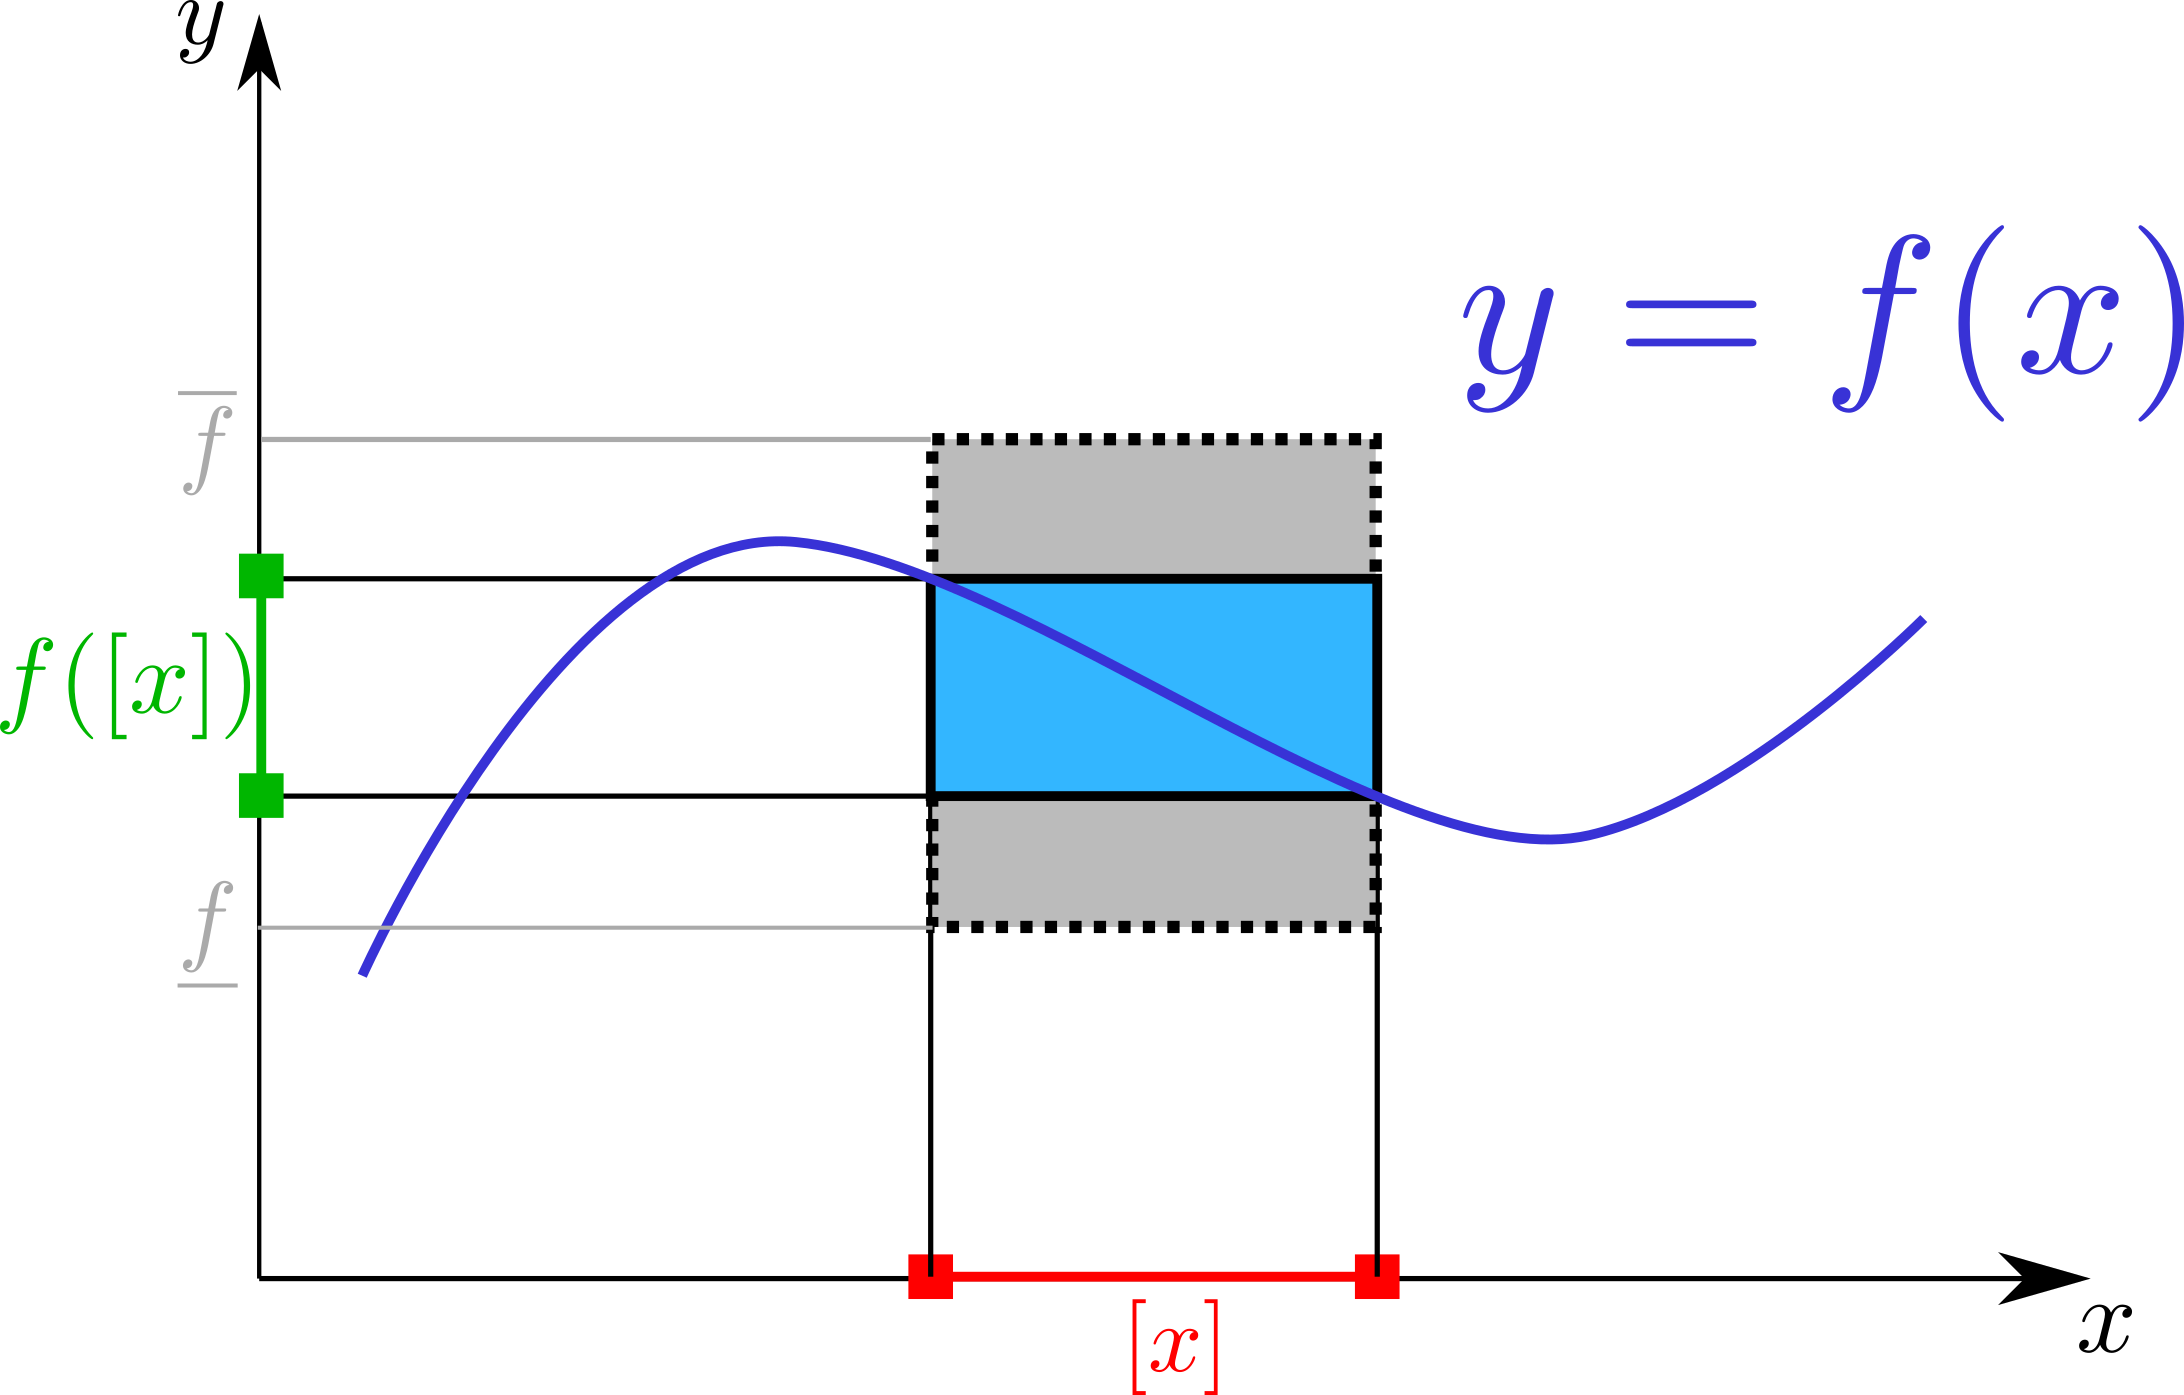
\includegraphics[scale=0.5]{intervaleval/function_eval_3.png}
  \caption{Fonction d'inclusion composée de moindre qualité}
  \label{fig:fct3}
\end{figure}

% Fonction d'inclusion par la forme centrée

\subsection{Arithmétique élémentaire}

Comme dit précédement, on peut construire les fonctions d'inclusions des fonctions necessaires pour n'importe quel problème en calcul par intervalle. Spécifiquement, il est utile de définir un certain nombre de fonctions de base permettant de former les blocs de construction pour la formation de fonctions plus complexes. On peut ainsi définir les opérateurs binaires (l'addition, la soustraction, la multiplication, \dots) ainsi que les opérateurs unaires (l'exponentielle, la puissance, le sinus, \dots).

\begin{ex}
  
  Un certain nombre de fonctions arithmétiques élémentaires peuvent être formulées :
  \begin{itemize}
    \item $[x_1] + [x_2] = [\underline{x_1} + \underline{x_2}, \overline{x_1} + \overline{x_2}]$
    \item $[x_1] - [x_2] = [\underline{x_1} - \overline{x_2}, \overline{x_1} - \underline{x_2}]$
    \item $[x_1] \times [x_2] = [\text{min}(\underline{x_1}\underline{x_2}, \underline{x_1}\overline{x_2}, \overline{x_1}\underline{x_2}, \overline{x_1}\overline{x_2}), \text{max}(\underline{x_1}\underline{x_2}, \underline{x_1}\overline{x_2}, \overline{x_1}\underline{x_2}, \overline{x_1}\overline{x_2})]$
    \item $[x]^2 = [0, \text{max}(\underline{x}^2, \overline{x}^2)]$
    \item $e^{[x]} = [e^{\underline{x}}, e^{\overline{x}}]$
    \item \dots
  \end{itemize}
\end{ex}

On peut étendre ces définitions à l'ensemble des fonctions strictements monotones: il est évident de se dire que, si une fonction $f(x)$ est strictement croissante, alors $[f]([x]) = [f(\underline{x}), f(\overline{x})]$, et de même pour une fonction décroissante. On peut alors construire des fonctions plus complexes, comme $f : x \mapsto x^3$ en découpant la définition de la fonction par morceaux.

\section{Optimisation avec les intervalles}
On met en place un algorithme d'optimisation utilisant le calcul par intervalle pour obtenir un encadrement garanti de la solution à notre problème.

On veut résoudre le problème $\max(f(x))$ tel que $g(x) \leq 0$, avec $f$ fonction coût et $g$ ensemble des contraintes. Avec le calcul par intervalle, on cherche à avoir un encadrement \textit{garanti} de la solution au problème. Le principe de base est de découper l'ensemble des entrées en un certain nombre de boites, dépendant de la précision que l'on veut, comme à la figure \ref{fig:optim1}. On choisit ensuite un $a$ solution admissible du problème suivant le théorème \ref{thm:solutionsup}.

\begin{theoreme}
  \label{thm:solutionsup}
  Soit un $a$ une solution admissible du problème $\max\limits_{x} f(x)$ tel que $g(x) \leq 0$ et $x^*$ la solution optimale, on a:
  \begin{align}
      sup([f]([x])) \leq f(a) \Rightarrow x^* \notin [x]
  \end{align}
\end{theoreme}

Cela nous permet d'éliminer directement de l'ensemble des solutions les boites dont la borne supérieure de l'image est inférieure à l'image de ce critère $a$, puisque garanties comme ne contenant pas l'optimum du problème. La figure \ref{fig:optim2} illustre cette élimination. \`A l'issue de cette étape, on voit qu'on obtient un ensemble plus restreint de boites garanties comme contenant la solution, et on peut itérer en choisissant au fur et à mesure un critère $a$ meilleur, et on arrive à un encadrement satisfaisant de la solution comme à la figure \ref{fig:optim3}.

\begin{figure}[H]
  \centering
  \begin{subfigure}[h]{0.3\textwidth}
      \centering
      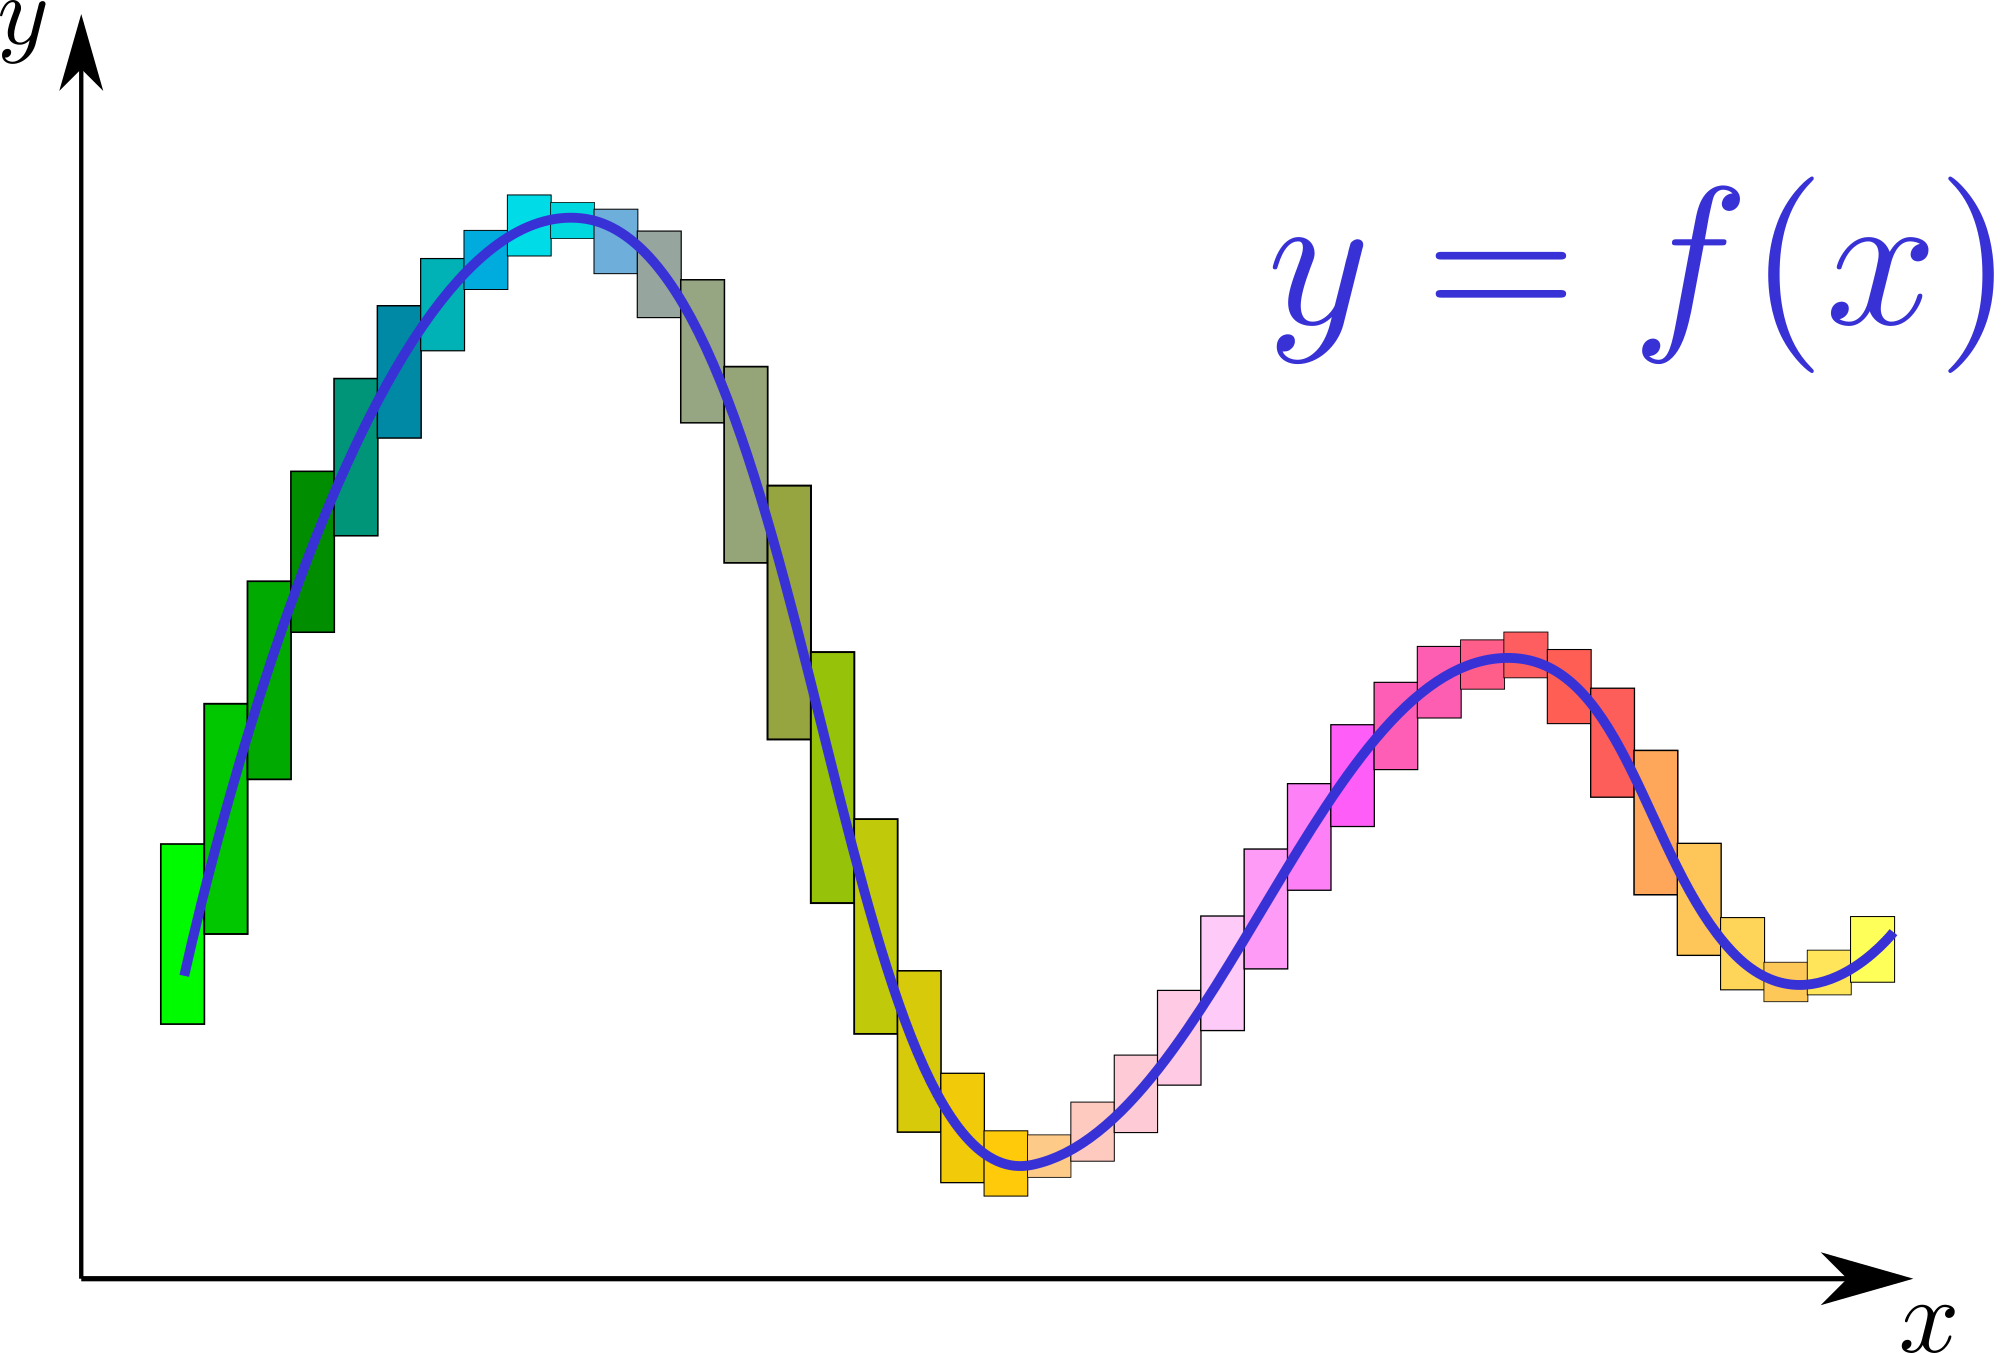
\includegraphics[scale=0.4]{AlgoOptim/function_optim_1.png}
      \caption{}
      \label{fig:optim1}
  \end{subfigure}
  \begin{subfigure}[h]{0.3\textwidth}
      \centering
      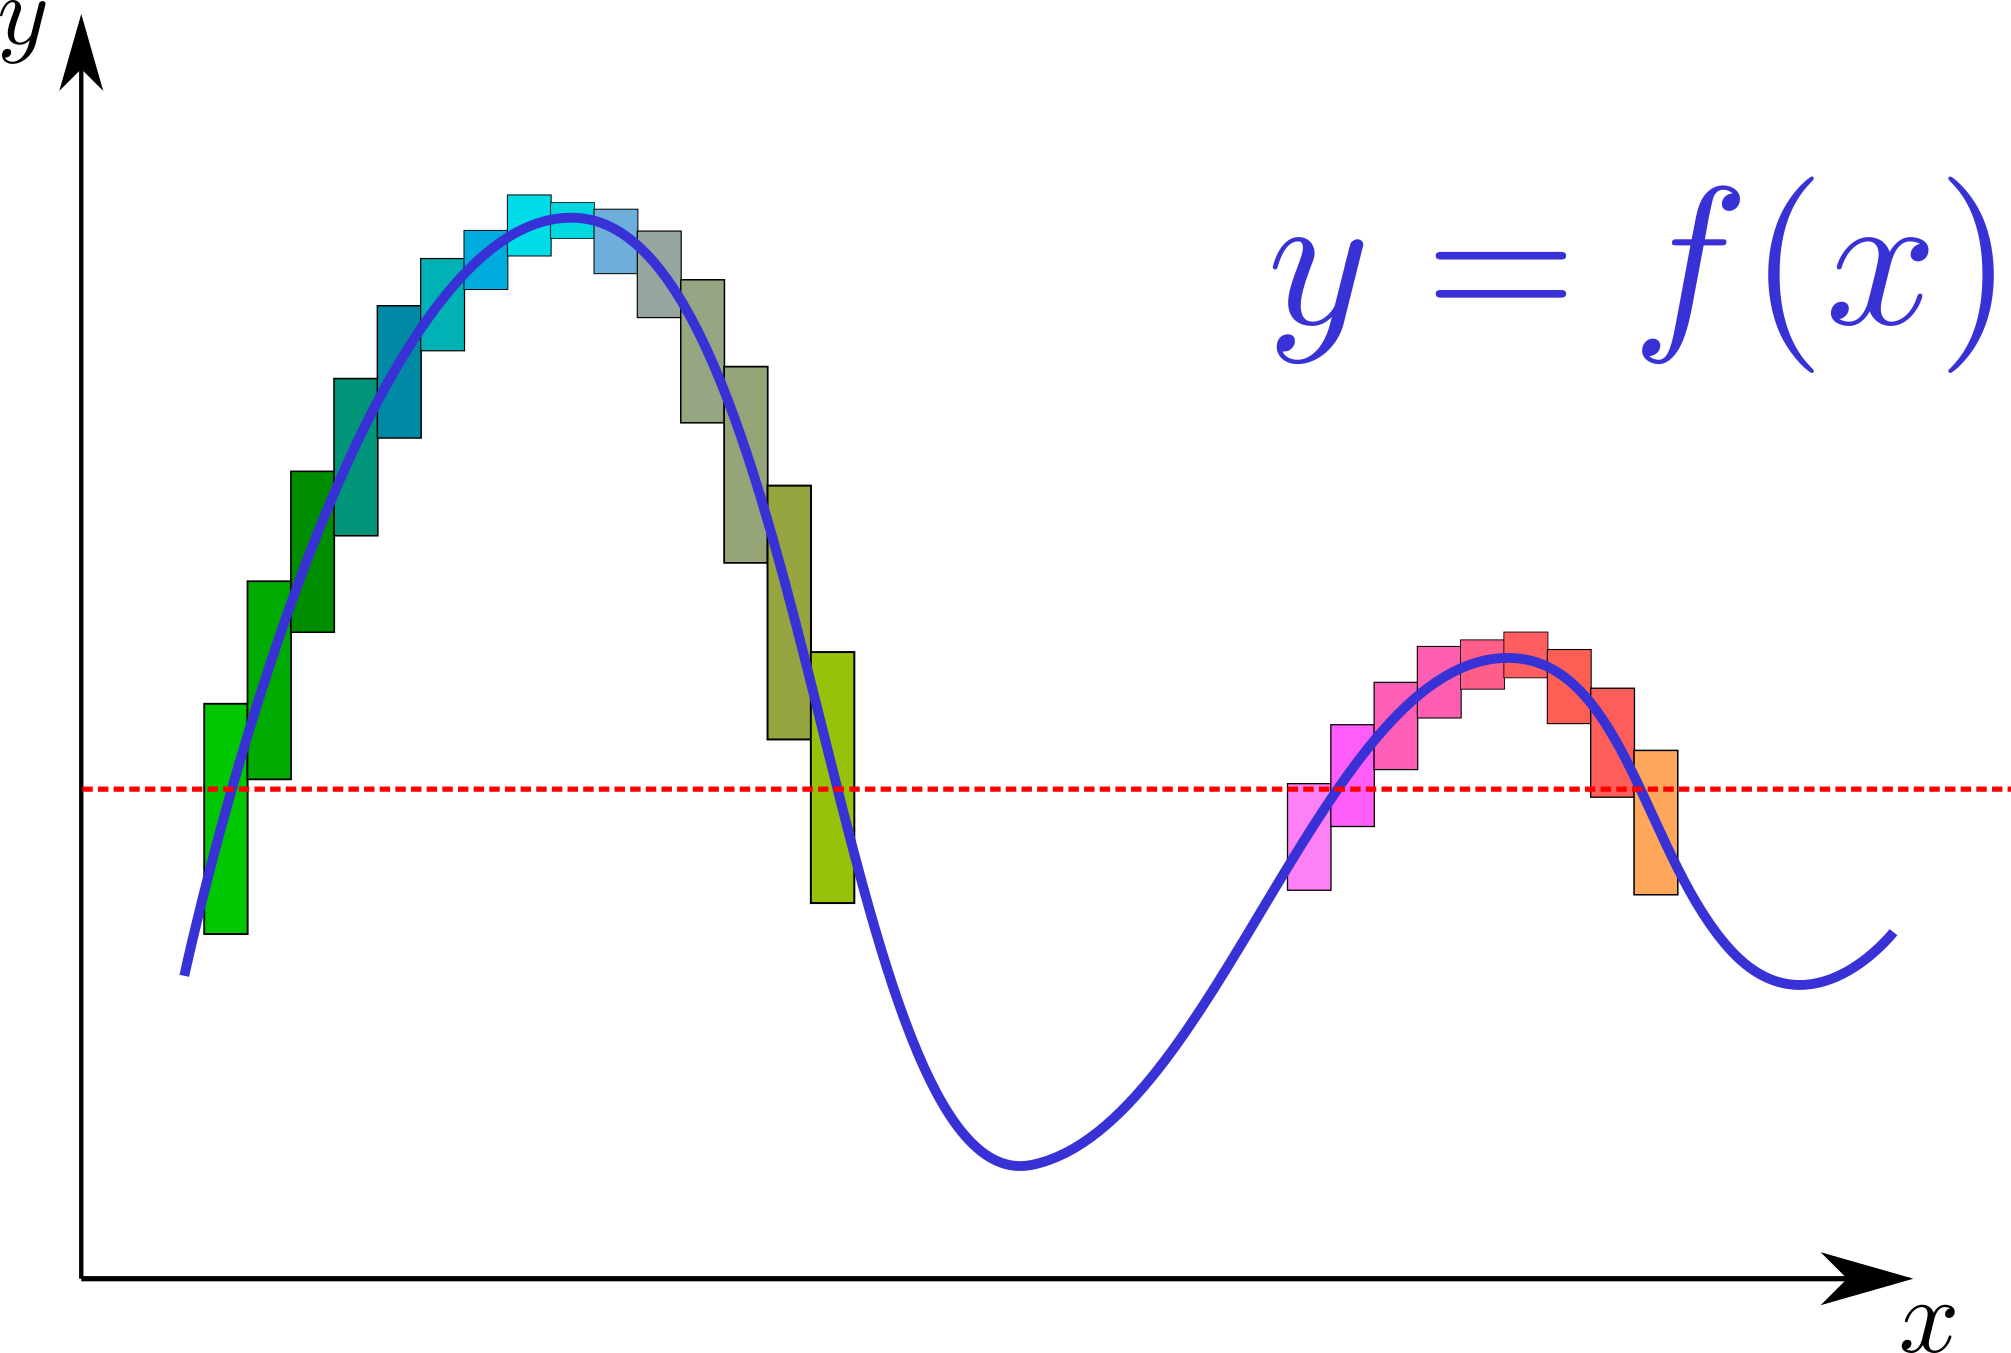
\includegraphics[scale=0.4]{AlgoOptim/function_optim_4.png}
      \caption{}
      \label{fig:optim2}
  \end{subfigure}
  \begin{subfigure}[h]{0.3\textwidth}
      \centering
      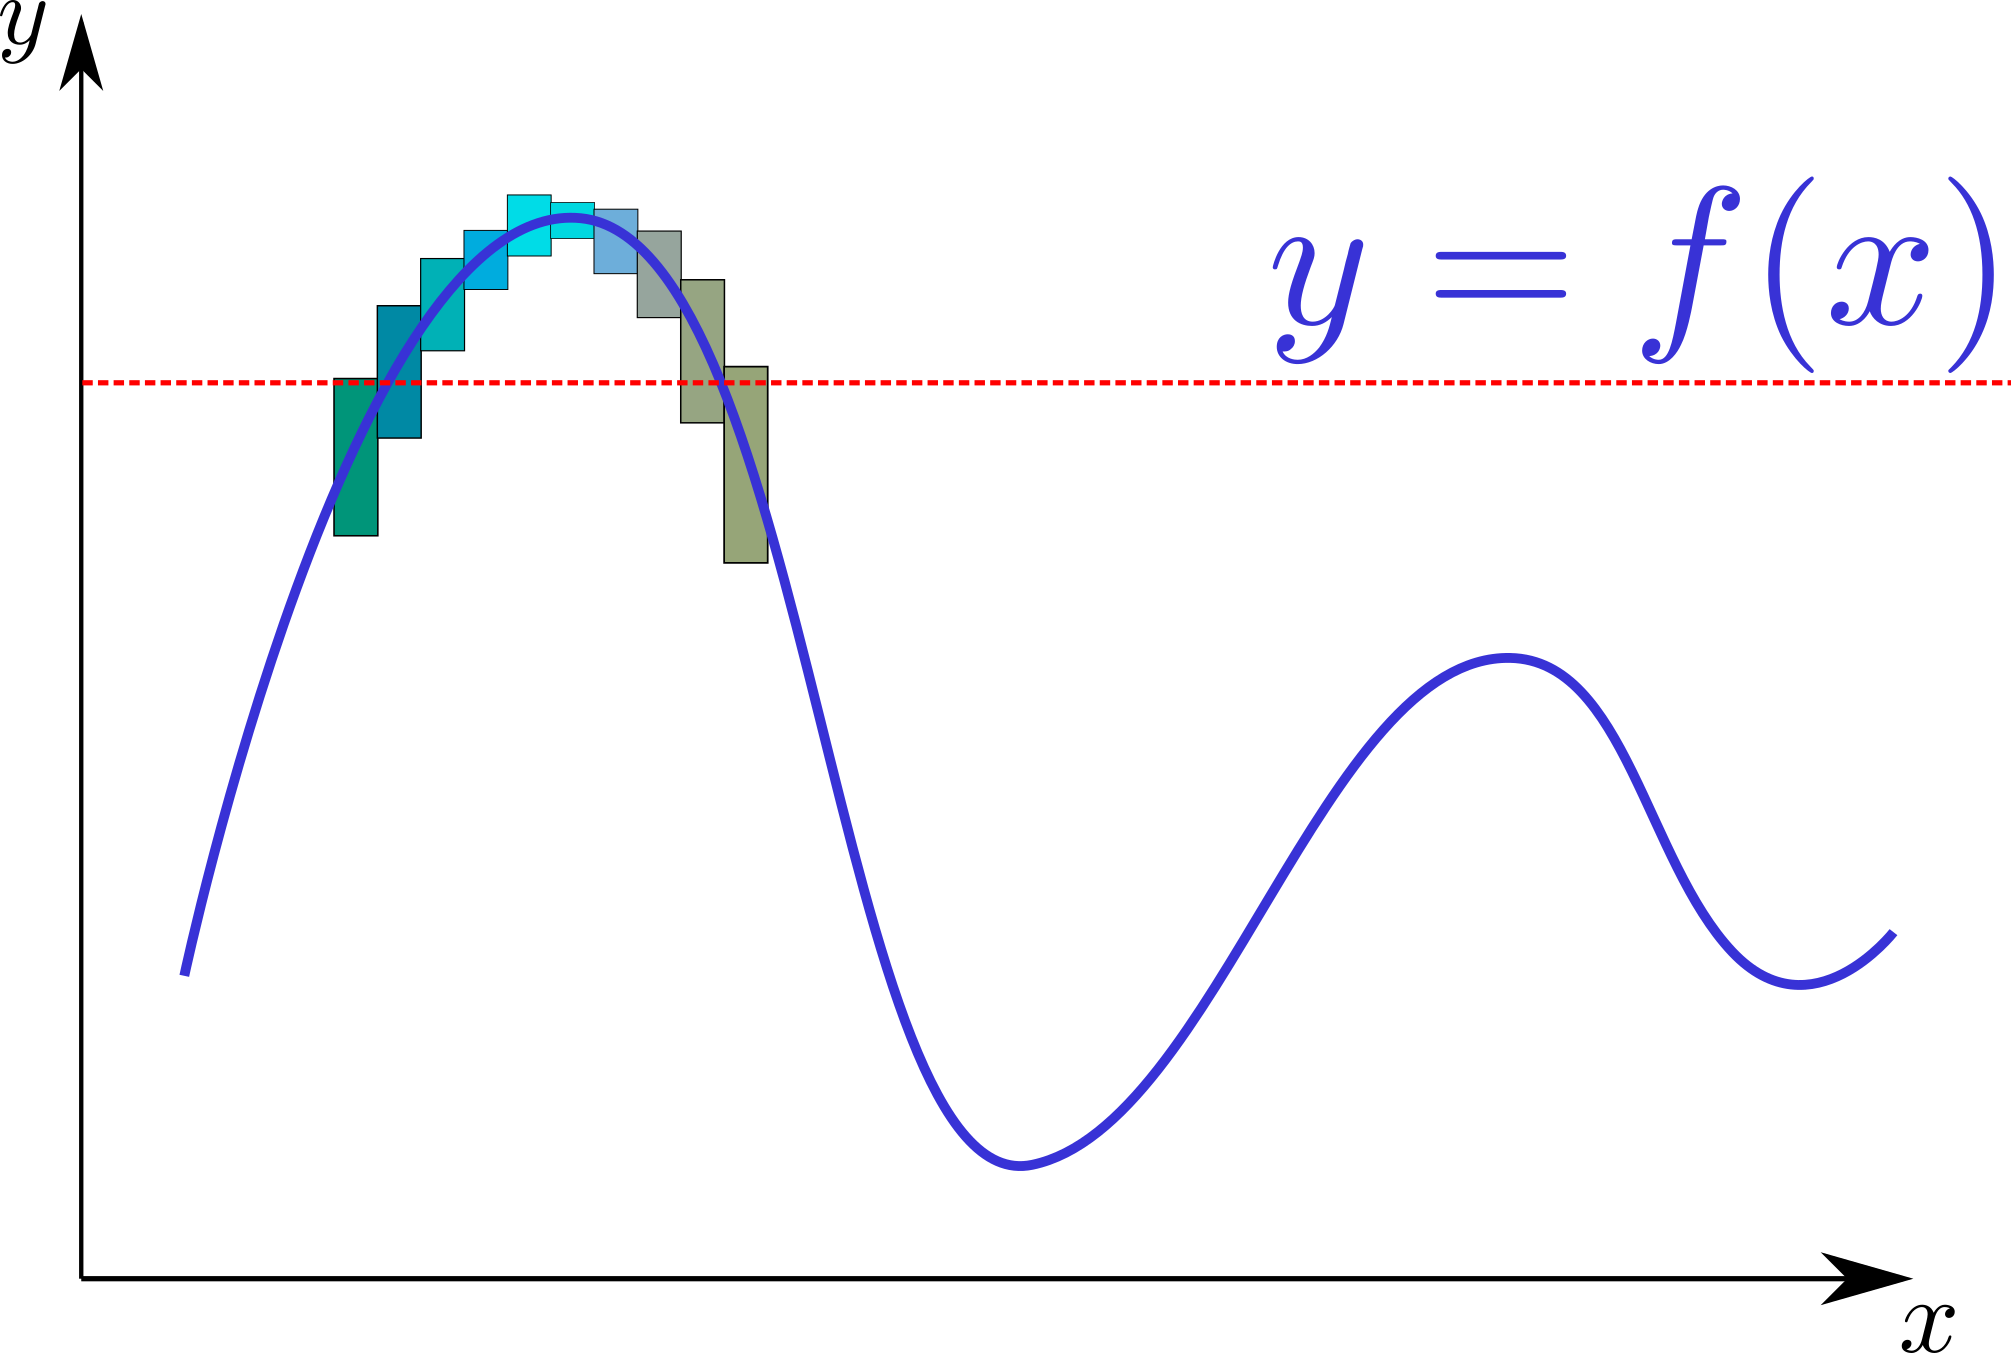
\includegraphics[scale=0.4]{AlgoOptim/function_optim_6.png}
      \caption{}
      \label{fig:optim3}
  \end{subfigure}
  \caption{Optimisation naïve}
\end{figure}

Cette méthode d'optimisation, "naive", permet d'obtenir un résultat satisfaisant mais va être rapidement limitée si on veut des précisions plus élevées. En effet, on va avoir très rapidement un très grand nombre de boites à traiter. On peut remarquer entre autres qu'un certain nombre de boites vont être dans des "régions" globales pouvant être éliminées (par exemple, sur la figure \ref{fig:optim2} on a tout le bas de la fonction qui pourrait être éliminé d'un coup). Cela nous amène à un algorithme plus avancé, présenté en \ref{fig:algomaxim}.

Au lieu de découper directement l'espace des entrées en un très grand nombre de boites, on va bisecter l'espace en deux boites, suivant l'axe le plus grand. On obtient deux boites, dont l'axe le plus grand aura été coupé en faisant $[x] \longrightarrow {[\underline{x}; (\overline{x} + \underline{x}) . 0.5], [(\overline{x} + \underline{x}) . 0.5; \overline{x}]}$. On considère la bisection par le milieu, mais on pourrait aussi utiliser des bisections plus avancées permettant d'accélérer l'algorithme.

Une fois obtenues ces deux boites, on peut évaluer la fonction d'inclusion et les contraintes, et décider de jeter les boites ne rentrant pas dans les contraintes. Sur l'ensemble des boites obtenues pour une itération, on effectue l'opération de recherche de critère décrit précédement, et on réitère sur les boites restantes. Cela permet d'éliminer rapidement les boites de grande dimension qui sont garanties ne comprenant pas l'optimum, et donc réduire considérablement le nombre de boites à traiter par la suite.

On considère l'algorithme fini quand on a obtenu une précision suffisante sur l'encadrement de la fonction ou des variables d'entrée, ou alors quand un certain nombre d'itérations ont été effectuées.

\begin{figure}[H]
    \begin{algorithm}[H]
        \SetAlgoLined
        \KwData{
          $[I_{init}]$ initial search box;
          $\epsilon$ stop criterion;
          $f$ cost function;
          $g$ constraints function;
        }
        \KwOut{
          $[f]$ bounds of best solution; $[I]$ solution box
        }
        \Begin{
          $\texttt{solutions}$ list of solution boxes\;
          Add $[I_{init}]$ to $\texttt{solutions}$\;
          $[f_{c}]$ current bounds of solutions\;
          \While{$\overline{f_{c}} - \underline{f_{c}} \geq \epsilon$}{
              $\texttt{currentSolutions}$ empty list of boxes\;
              \tcc{Bisect, evaluate cost, manage constraints}
              \ForAll{$\texttt{sol}$ in $\texttt{solutions}$}{
                    $[\texttt{left}], [\texttt{right}] \longleftarrow \texttt{bisect}(\texttt{sol})$\;
                    \If{$\texttt{g}([\texttt{left}])$ is valid}{
                        Add $[\texttt{left}]$ to $\texttt{currentSolutions}$\;
                    }
                    \If{$\texttt{g}([\texttt{right}])$ is valid}{
                        Add $[\texttt{right}]$ to $\texttt{currentSolutions}$\;
                    }
              }
              \tcc{Remove boxes certified not to contain maximum}
              Evaluate $[f]$ for all $[\texttt{currentSolutions}]$\;
              $f_{best}$ best $f(\texttt{sol}.\texttt{mid})$ in all $[f]$ \;
              Remove all $[\texttt{sol}]$ in $[\texttt{currentSolutions}]$ where $sup([f]([\texttt{sol}])) \leq f_{best}$\;
              $\texttt{solutions} \longleftarrow \texttt{currentSolutions}$
          }
          \Return{$\texttt{solutions}, [f_{c}]$}
        }
      \end{algorithm}

    \caption{Algorithme de maximisation par le calcul par intervalle}
    \label{fig:algomaxim}
\end{figure}

\section{Implémentation}

L'algorithme \ref{fig:algomaxim} a été implémenté en C\# (dotnet 5) sur la base de la librairie \href{https://github.com/selmaohneh/IntSharp}{IntSharp} modifiée pour répondre à nos besoins (rajout de l'intervalle vide, de la fonction $x\log(x)$, des intervalles booléens, \dots). Une interface graphique basique utilisant Blazor a été mise en place pour faciliter la visualisation de l'optimisation et des différents problèmes rencontrés lors du développement. L'ensemble du projet est disponible sur \url{https://github.com/PierreEngelstein/IntervalEval}. La solution est organisée en plusieurs modules:

\begin{itemize}
  \item \texttt{IntervalEval} qui fourni la librairie de base pour le calcul par intervalle et l'optimisation;
  \item \texttt{IntervalEval.Front} est l'interface web basique développée avec le framework Blazor Server;
  \item \texttt{IntervalEval.Optimizer} est une interface en ligne de commande pour le problème spécifique détaillé dans ce rapport;
  \item \texttt{IntervalEval.FrontConsole} est une interface en ligne de commande codée pour tester le problème à trois états quantiques d'entrée, pour tester les performances sur un problème en plus haute dimension;
  \item \texttt{IntervalEval.Tests} fourni un ensemble de tests unitaires pour le bon fonctionnement de la librairie d'intervalle.
\end{itemize}

\chapter{Construction d'un détecteur optimal}

On présente ici le détail du problème de la détection optimale quantique avec le critère de l'information mutuelle. 

\section{Formulation du problème}
Le problème de la détection d'état quantique porte sur un ensemble de $m$ états quantiques représentés par les opérateurs densité $\{\rho_i \; , \; 1 \leq i \leq m\}$ munis des probabilités à priori $\{p_i \geq 0 \; , \; 1 \leq i \leq m \}$. L'objectif est d'obtenir un ensemble de $m$ opérateurs de mesure $\{\Pi_j \; , \; 1 \leq i \leq m\}$ permettant de mesurer le mieux possible par rapport aux probabilités les états d'entrée qui nous arrivent.

Les opérateurs $\rho_i$ et $\Pi_i$ sont des matrices Hermitiennes semi-définies positives, de la forme $\begin{bmatrix}a & b+ic \\ b-ic & d \end{bmatrix}$.

Plusieurs critères ont été proposés à optimiser afin de construire ces détecteurs optimaux. D'une part, on a la possibilité de travailler sur la minimisation de l'erreur quadratique de mesure \cite{Eldar01} ou la maximisation de la probabilité de détection correcte \cite{Eldar03c}. D'autre part, et c'est ce sur quoi nous avons travaillé, on peut considérer le critère de l'information mutuelle comme critère à maximiser \cite{Davies78}. Ce critère indique la dépendance de deux variables aléatoires entre elles, il permet dans notre cas de bien caractériser la quantité d'information qu'on peut retirer des états d'entrée en ayant les opérateurs de mesure
\medbreak
L'information mutuelle de deux variables aléatoires $X$ et $Y$ a été formulée par Shannon en 1948 \cite{Shannon48}. Elle est donnée par:

\begin{align}
    I(X;Y) = \displaystyle \sum_{y \in Y} \displaystyle \sum_{x \in X} p_{(X, Y)}(x, y) \log \big(\frac{p_{(X, Y)}(x, y)}{p_X(x) p_Y(y)}\big),
\end{align}

mais peut aussi être écrite en fonction des entropies des variables aléatoires:

\begin{align}
    I(X; Y) &= H(X) - H(X | Y) \\
            &= H(Y) - H(Y | X) \\
            &= H(X) + H(Y) - H(X, Y).
\end{align}

Avec $H(X)$ entropie marginale de $X$, $H(Y)$ entropie marginale de $Y$, $H(X|Y)$ entropie conditionelle de $X$ sachant $Y$ et enfin $H(X, Y)$ entropie jointe de $X$ et $Y$. On peut utiliser indifférement $\log_2$, $\log_{10}$ ou $\ln$ pour le logarithme, le changement étant à une constante près. On utilise par la suite le logarithme base exponentielle pour l'ensemble des calculs.

Dans le cas classique, les entropies marginales, conditionnelles et jointes sont définies par: 

\begin{align}
    H(X) &= -\displaystyle \sum_{x \in X} p(x) \log(p(x)) , \\
    H(Y) &= -\displaystyle \sum_{y \in Y} p(y) \log(p(y)) , \\
    H(X, Y) &= -\displaystyle \sum_{x \in X} \displaystyle \sum_{y \in Y} p(x, y) \log(p(x, y)), \\
    H(Y|X) &= -\displaystyle \sum_{x \in X, y \in Y} p(x, y) \log \big(\frac{p(x, y)}{p(x)}\big)
\end{align}

Dans le cas quantique, les formules restent les mêmes, mais on exprime les probabilités des variables en fonction des valeurs des états quantiques d'entrée.

En fonction d'un état d'entrée $\rho_i$ de probabilité préalable $p_i$, et d'un opérateur de sortie $\Pi_i$, on peut définir leur probabilité jointe :

\begin{align}
    p(X = \rho_i, Y = \Pi_i) = p_i \tr(\rho_i \Pi_i).
\end{align}

On en déduit les probabilités marginales:

\begin{align}
    p(X = \rho_i) = \displaystyle \sum_{j}p_i \tr(\rho_i \Pi_j)  \\
    p(Y = \Pi_j) = \displaystyle \sum_{i}p_i \tr(\rho_i \Pi_j),
\end{align}

Et les probabilités conditionelles:

\begin{align}
    P(Y=\Pi_j | X=\rho_i) = \frac{\tr(\rho_i \Pi_j)}{\displaystyle \sum_{k} \tr(\rho_i \Pi_k)}
\end{align}

L'information mutuelle pour notre problème peut donc être ré-écrite de la façon suivante, en utilisant $\alpha_{ij} = \tr(\rho_i \Pi_j)$ :

\begin{align}
    \label{eq:mi}
    I(\rho; \Pi) &= H(\rho) + H(\Pi) - H(\rho, \Pi) \nonumber \\
    &= - \displaystyle \sum_{i=1}^{m} \big(\displaystyle \sum_{j=1}^{m} \alpha_{ij} \big) \log \big( \displaystyle \sum_{j=1}^{m} \alpha_{ij} \big) - \displaystyle \sum_{i=1}^{m} \big(\displaystyle \sum_{j=1}^{m} \alpha_{ji} \big) \log \big( \displaystyle \sum_{j=1}^{m} \alpha_{ji}\big) + \displaystyle \sum_{i=1}^{m} \displaystyle \sum_{j=1}^{m} \alpha_{ij} \log( \alpha_{ij} )
\end{align}

On peut aussi exprimer l'information mutuelle en fonction de l'entropie conditionnelle, mais il est plus efficace d'utiliser celle donnée à l'équation \ref{eq:mi} pour la résolution numérique.

Le problème se formule comme un problème de maximization de l'information mutuelle: on cherche à maximiser l'information qu'on peut obtenir sur $\rho_i$ quand on a les opérateurs de mesure $\Pi_i$:

\begin{align}
    \max\limits_{\Pi} I(\rho, \Pi)
\end{align}
tel que :

\begin{align}
    \Pi_j \succeq 0 \quad 1 \leq j \leq m \label{eq:contrainte_sdp} \\
    \displaystyle \sum_{j=1}^{m} \Pi_j = I \label{eq:contrainte_somme_id}
\end{align}

La contrainte \ref{eq:contrainte_sdp} correspond à la semi-définition positive des opérateurs de mesure $\Pi_j$. Enfin, la contrainte \ref{eq:contrainte_somme_id} permet d'obtenir des opérateurs de mesure cohérents pour que les probabilités de mesure $p(j) = \tr (\rho \Pi_j)$ soient positives et se somment à 1.

On est en présence d'une fonction convexe, et les contraintes engendrent un ensemble admissible convexe. C'est le cas idéal lors d'une minimisation, mais le problème est une maximisation, de même difficulté qu'une minimisation concave, on ne peut donc pas juste faire une descente de gradient pour le résoudre. On peut utiliser un certain nombre de méthodes approximatives, nous utilisons le calcul par intervalle afin d'obtenir un résultat sûr dans un intervalle.

\section{Convexité de l'information mutuelle}
Davies considère en 1978 que l'information mutuelle pour ce problème peut être considérée comme étant convexe, simplifiant la résolution du problème en ayant à chercher le maximum sur les bords. On s'intéresse ici à l'étude de cette convexité.

Dans son article, Davies regroupe les traces et probabilités sous une seule variable $P_{ij} = p_i \tr(\rho_i \Pi_j)$. Ces coefficients $P_{ij}$ forment une matrice des probabilités, telle que :

\begin{align}
    \displaystyle \sum_{ij} P_{ij} = 1, \\
    \displaystyle \sum_{i}  P_{ij} = p_i.
\end{align}
L'information mutuelle s'écrit donc :

\begin{align}
    I(P) = \displaystyle \sum_{i} H(\displaystyle \sum_{j}P_{ij}) + \displaystyle \sum_{j} H(\displaystyle \sum_{i}P_{ij}) -  \displaystyle \sum_{ij} H(P_{ij}) 
\end{align}

La fonction $H(x) = -x \log(x)$ est convexe, et donc $I$ est convexe par rapport à la matrice des probabilités $P$. La figure \ref{fig:mi_convex} illustre cette fonction en fixant $p_1 = 0.3$ et $p_2 = 0.7$.

\begin{figure}[h]
    \centering
    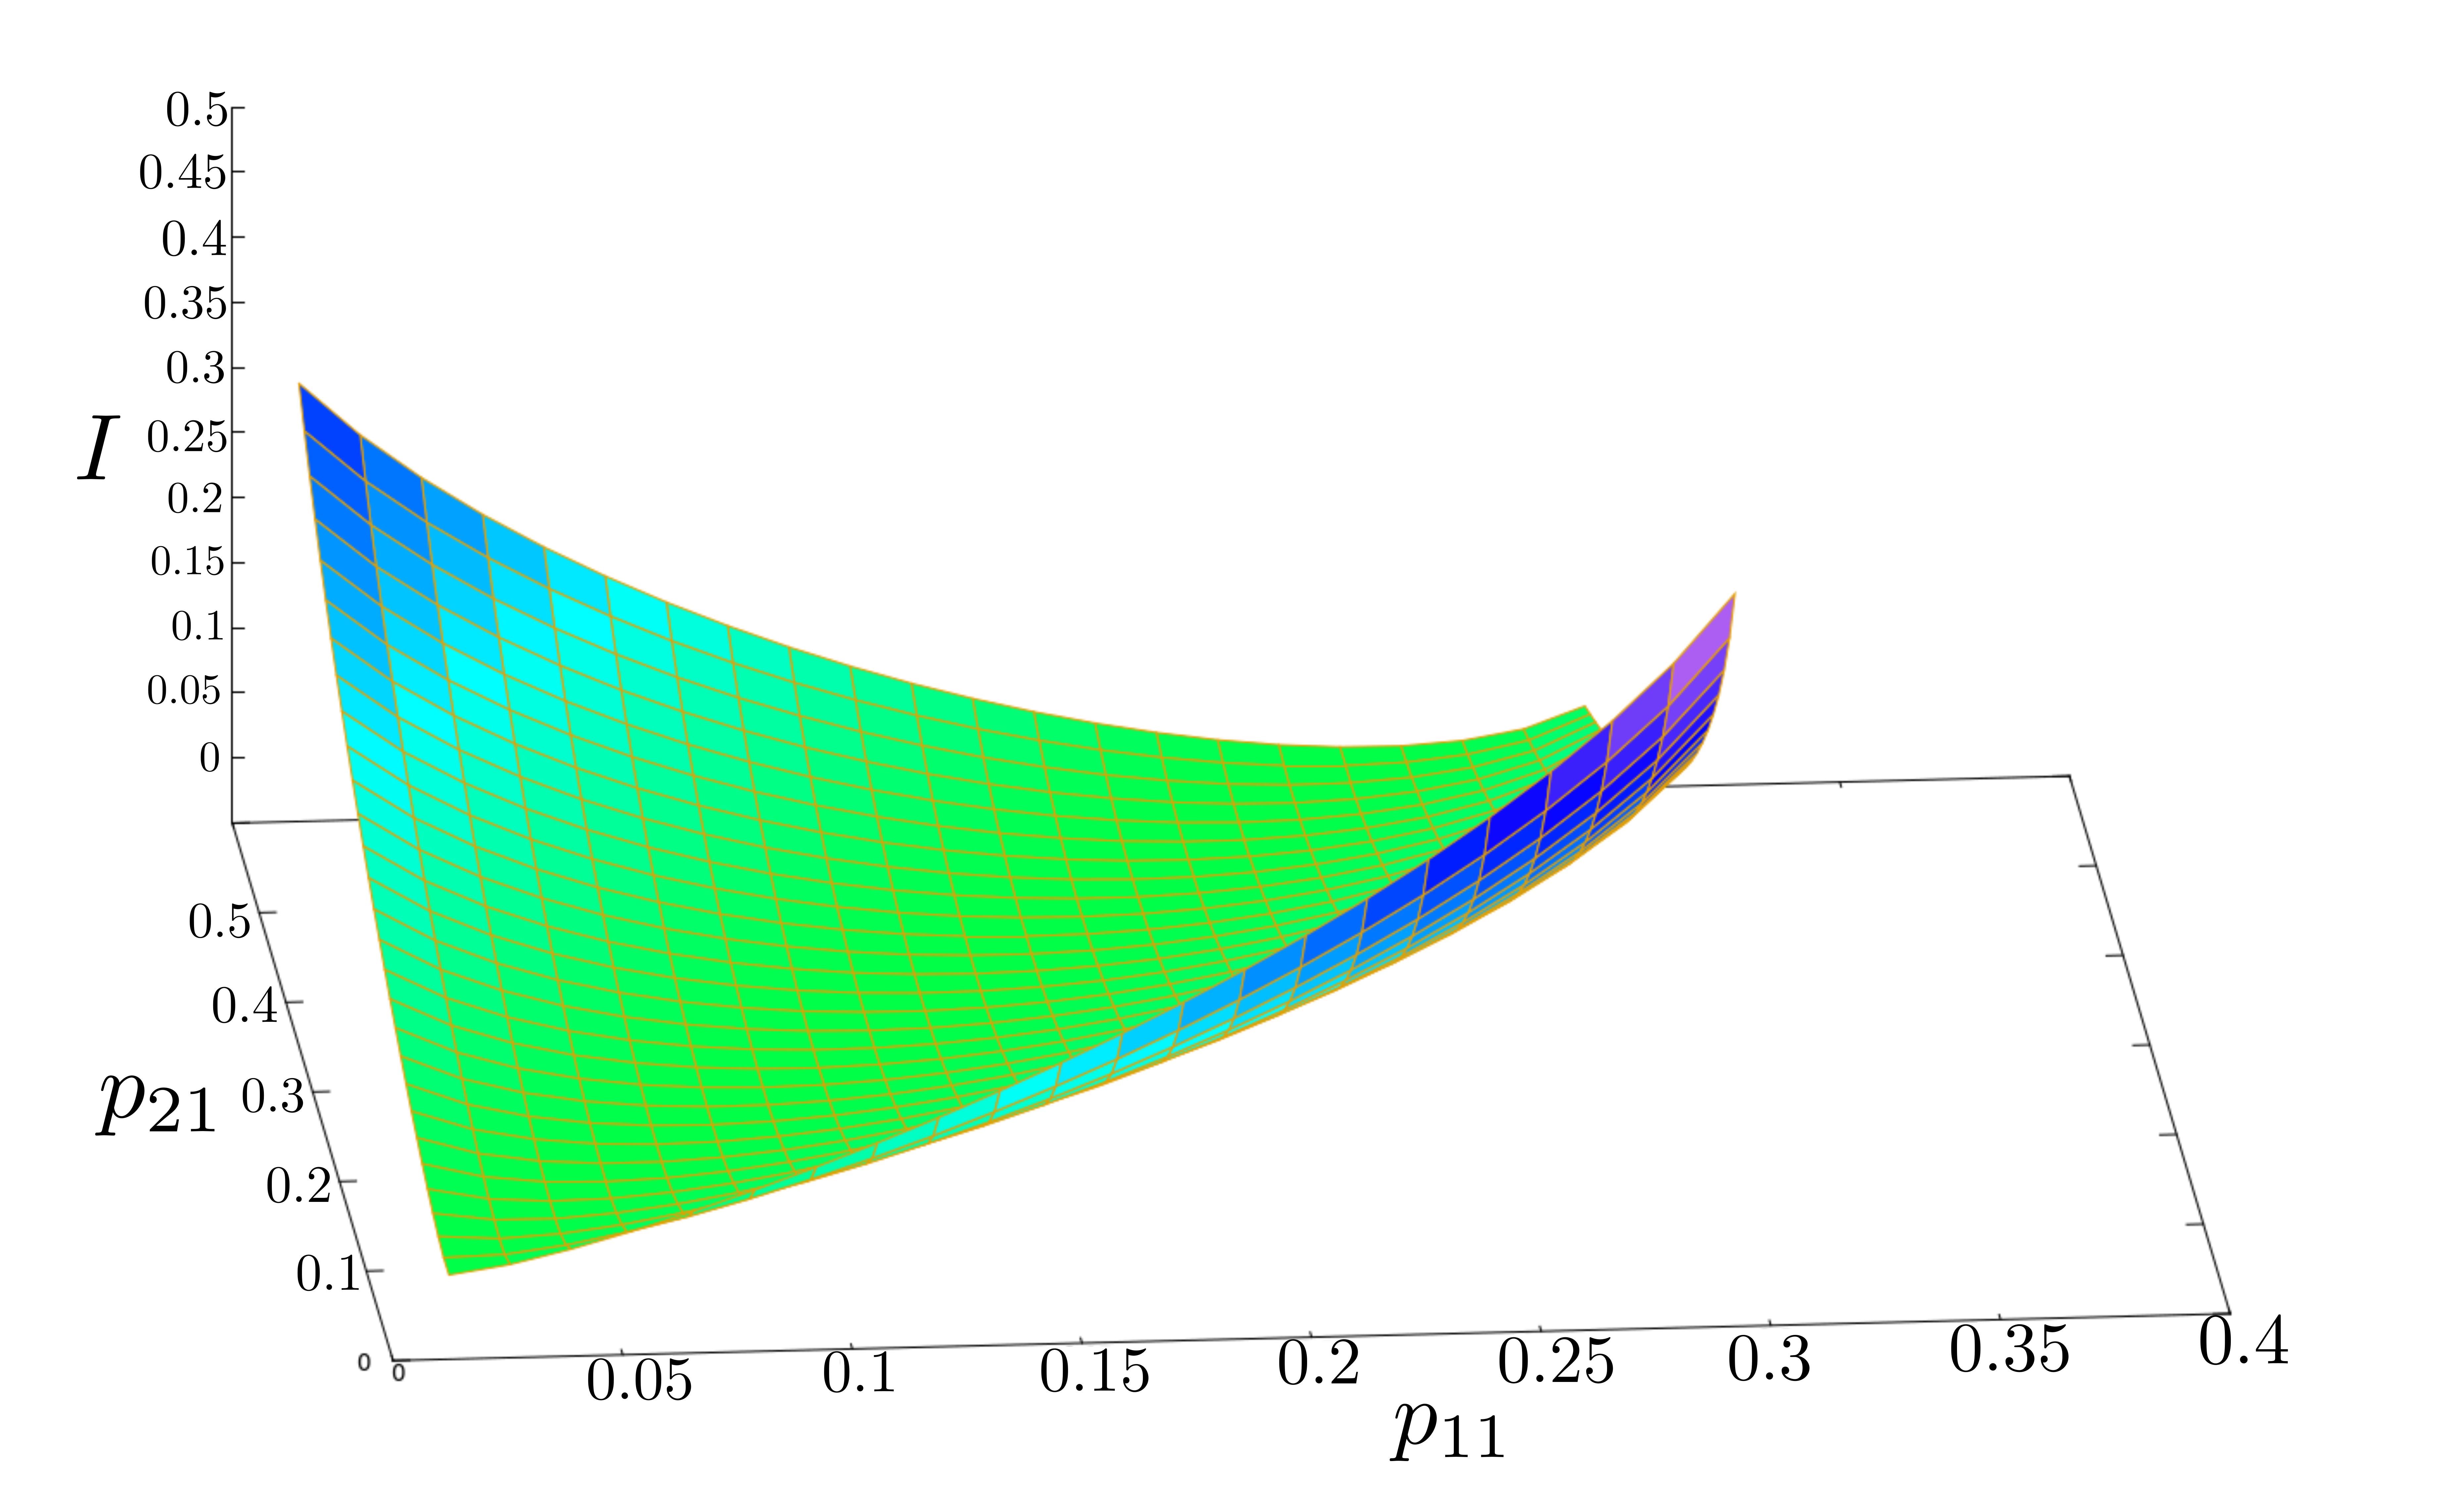
\includegraphics[scale=0.2]{pb/MI_convex.png}
    \caption{Information mutuelle par rapport à la matrice de probabilités}
    \label{fig:mi_convex}
\end{figure}

La convexité semble bien vraie par rapport à $P$, mais on cherche à optimiser les matrices $\Pi_j$. La matrice $P$ comporte les traces de la multiplication $\rho_i \Pi_j$, qui est linéaire par rapport aux coefficients de $\Pi_j$. Si la fonction $I(P)$ est convexe par rapport à $P$, alors elle l'est par rapport aux $\Pi_j$, grace à la linéarité.

Quand on trace la même fonction mais par rapport aux variables $\Pi_{k_{ij}}$, en se fixant dans un espace 2 dimensions, on s'apperçoit que la fonction n'est pas correctement définie sur les bords. Ceci est dû au fait que $x\log(x)$ n'est pas définit pour $x < 0$, ce qui fausse ou bloque les calculs, suivant l'implémentation. Le détail de notre implémentation est expliqué en \ref{fig:xlog}. % TODO: change this to subsubsection reference !

\medbreak

\section{Formulation des contraintes}

La définition du problème permet de résoudre notament les cas immédiats des opérateurs de densité orthogonaux, mais la résolution devient très lente lorsqu'on passe à d'autres cas non orthogonaux. On rajoute des conditions au problème pour accélérer la résolution.

Le premier élément à simplifier est l'expression de l'entropie marginale de $X=\rho_i$. En effet, nous l'avons exprimé en fonction de la trace de la multiplication matricielle, mais on peut reprendre la définition donnée lors du cas classique qui dit que $ H(X) = -\displaystyle \sum_{x \in X} p(x) \log(p(x))$. Le problème nous indique que nous connaissons les probabilités préalables des états d'entrée, on peut donc directement exprimer cette entropie en fonction de ces données et donc sans les variables de sortie $\Pi_i$.

Ensuite, on sait que les opérateurs de mesure se somment à l'identité. Cela signifie d'une part qu'on peut passer d'un problème à $m$ matrices à un problème à $m-1$ matrices pour $m \geq 2$. Les matrices étant carrées de dimension $n$, on passe de $m \times n^2$ variables à $(m - 1) \times n^2$ variables, ce qui est non négligeable.

De plus, le problème et les contraintes sont symmétriques, on peut intervertir les $\Pi_j$ sans influencer le résultat de la fonction coût. Cela nous permet de couper le problème au moins en deux pour réduire à nouveau le temps de calcul. Du fait de la somme à l'identité, on peut ajouter en contrainte que $\Pi_{1_{1, 1}} \leq \frac{1}{m}$ pour $m$ opérateurs de mesure, puis $\Pi_{2_{1, 1}} \leq \frac{1}{m-1}$, etc.

Enfin, pour rappel, les opérateurs de mesure sont des opérateurs densité, qui ne sont pas necessairement purs. Pour qu'ils soient purs, il faudrait entre autre que $\tr(\Pi_i) = 1$. On peut considérer qu'on restreint le problème à un cas purs, et dans ce cas rajouter la contrainte que la somme des éléments diagonaux des opérateurs de mesure doit sommer à 1. Cela permet soit de retirer une variable par matrice densité au problème, en l'exprimant par $x_{n+1} = 1 - \displaystyle \sum_{i}^{n} x_i$ avec les $x_i$ éléments diagonaux de l'opérateur densité, ce qui nécessite une reformulation du problème, soit l'ajout de la contrainte.

\medbreak

\section{Résolution avec \texttt{ibex}}

Pour la résolution de ce problème, utilisons la librairie \texttt{ibex} permettant de faire du calcul par intervale, et possède entre autres un outil d'optimisation, \texttt{ibexopt}. Le problème est formulé avec un langage dédié, \texttt{minibex}. Nous avons eu besoin de définir un opérateur additionnel à ceux présents, l'opérateur \texttt{xlog} permettant d'effectuer l'opération $x \times \log(x)$ en redéfinissant $0 \times \log(0) = 0$ pour que les intervalles ne tombent pas à l'infiniquand ils contiennent 0. De plus, \texttt{minibex} ne considère que des problèmes de minimisation, on ré-écrit le problème en prenant la fonction coût opposée : $\max f(x) \Leftrightarrow \min -f(x)$.
\medbreak
Le premier test effectué est sur le cas de deux états d'entrée $\ket{\psi_1} = \ket{0}$ et $\ket{\psi_2} = \ket{1}$ ayant pour probabilité respective $p_1 = 0.1$ et $p_2 = 0.9$. Le résultat théorique est connu: les états étant orthogonaux, on doit obtenir les opérateurs de mesure égaux aux opérateurs densité d'entrée. On obtient bien avec \texttt{ibex} les opérateurs suivant:

$\Pi_1 = \begin{bmatrix} 0 & 0 \\ 0 & 1\end{bmatrix} , \quad \Pi_2 = \begin{bmatrix} 1 & 0 \\ 0 & 0\end{bmatrix},$

qui correspondent bien à deux opérateurs de mesure orthogonaux. Dans ce cas, l'information mutuelle est comprise dans l'intervalle $I(\rho, \Pi) \in [0.3250, 0.3254]$, avec un temps de calcul de 8.6 millisecondes.
\medbreak
Le deuxième cas qu'on peut présenter est le suivant: $\ket{\psi_1} = \ket{0}$ et $\ket{\psi_1} = \ket{+}$ avec comme probabilité respectives $p_1 = 0.1$ et $p_2 = 0.9$. Le résultat théorique n'est pas donné, et on obtient avec \texttt{ibex} le résultat suivant:

$\Pi_1 = \begin{bmatrix} 0.445 & 0.497 \\ 0.497 & 0.555\end{bmatrix} , \quad \Pi_2 = \begin{bmatrix} 0.555 & -0.497 \\ -0.497 & 0.445\end{bmatrix},$

avec une information mutuelle comprise dans l'intervalle $I(\rho, \Pi) \in [0.1348, 0.1349]$, et un temps de calcul de 0.79 secondes.

% On voit bien avec ces deux exemples l'augmentation radicale du temps de calcul quand on passe d'un problème simple, même orthogonal, à un problème plus compliqué.

En revanche, ibex ralentit fortement dès qu'on sort des cas simples présentés si-dessus, et notament quand on retire la restriction des opérateurs de mesure à des opérateurs densité purs (de trace unitaire). Deux éléments importants sont à l'origine du problème. Tout d'abord, en analysant l'utilisation des ressources cpu lors de la résolution d'un problème, on voit qu'un seul thread est utilisé par \texttt{ibexopt}. Les algorithmes d'optimisation peuvent être parallélisés, et dans le cas de processeurs à plusieurs c\oe urs on pourrait avoir un gain de performance conséquent. Le deuxième élément est en lien avec la convexité de la fonction coût évoqué précédement. On eut alors se limiter aux extremités de la fonction coût pour réduire le nombre de calculs à effectuer. Il faudrait alors implémenter la condition $0 \in [\texttt{grad}]([f])$, ce qui n'est pas prévu de base dans \texttt{ibexopt}.


\section{Exemple}

Prenons le cas de deux états quantiques:

\begin{align}
    \ket{\psi_1} = \begin{bmatrix}\frac{1}{3} \\ \frac{2 \sqrt{2}}{3}\end{bmatrix} , \quad \ket{\psi_2} = \begin{bmatrix}\frac{1}{\sqrt{2}} \\ \frac{1}{\sqrt{2}}\end{bmatrix},
\end{align}
avec les probabilités préalables 
\begin{align}
    p(\ket{\psi_1}) = 0.1, \quad p(\ket{\psi_2}) = 0.9.
\end{align}

Ces deux états peuvent être réécris sous la forme d'opérateurs densité $\rho_1 = \begin{bmatrix}\frac{1}{9} && \frac{2 \sqrt{2}}{9} \\ \frac{2 \sqrt{2}}{9} && \frac{8}{9} \end{bmatrix}$ et $\rho_2 = \begin{bmatrix}\frac{1}{2} && \frac{1}{2} \\ \frac{1}{2} && \frac{1}{2} \end{bmatrix}$.

Le problème est de trouver les deux opérateurs densité optimaux au sens de l'information mutuelle. On considère le problème comme ne possédant pas de termes complexes sur les antidiagonaux, et l'équation \ref{eq:contrainte_somme_id} nous permet de réduire le problème à trois variables seulement $\{a_1, b_1, d_1\}$ :

\begin{align}
    \Pi_1 &= \begin{bmatrix}a_1 && b_1 + ic_1 \\ b_1 - ic_1 && d_1\end{bmatrix} = \begin{bmatrix}a_1 && b_1 \\ b_1 && d_1\end{bmatrix} \\
    \Pi_2 &= I - \Pi_1 = \begin{bmatrix}1 - a_1 && -b_1 \\ -b_1 && 1 - d_1\end{bmatrix}
\end{align}

On pose ensuite les contraintes sur ces variables. Tout d'abord, ces variables sont définies sur ces bornes spécifiques: $a_1 \in [0, 0.5]$, $b_1 \in [-1, 1]$, $d_1 \in [0, 1]$. La détermination de la semi-définition positive passe par les diagnonales et le déterminant strictement positifs, d'une part avec les bornes précédentes et d'autre part avec deux nouvelles contraintes sur les 3 variables.
Le problème s'écrit donc :

\begin{align}
    \max\limits_{a_1, b_1, d_1} I(a_1, b_1, d_1) , \nonumber
\end{align}
tel que :
\begin{align}
    &a_1 \in [0, 0.5] , b_1 \in [-1, 1] , d_1 \in [0, 1] , \nonumber \\
    &a_1 * d_1 - b_1^2 \geq 0 , \nonumber \\
    &(1-a_1) * (1-d_1) - b_1^2 \geq 0. \nonumber
\end{align}

La résolution avec \texttt{ibex} ou avec notre solveur donne les deux opérateurs de mesure suivants: 

\begin{align}
    \Pi_1 = \begin{bmatrix}0.456 && -0.498 \\ -0.498 && 0.544\end{bmatrix}, \quad \Pi_2 = \begin{bmatrix}0.544 && 0.498 \\ 0.498 && 0.456\end{bmatrix},
\end{align}

Avec une information mutuelle $I(a_1, b_1, d_1) = 0.04723$. Notre solveur résout le problème en $6.4$ secondes pour une précision sur $I$ de $1 \times 10^{-5}$, et \texttt{ibexopt} résout en $88.3$ secondes pour une précision sur $I$ de $4\times 10^{-5}$.

% \input{includes/chap-05-perpectives.tex}
% \chapter{Ouverture vers le stage}

A la suite de ce travail, un certain nombre de questions restent ouvertes et serviront de pistes de travail pour le stage qui suit:

\begin{itemize}
    \item Sur la construction effective des circuits, est-il optimal de décomposer le circuit en portes élémentaires CNOT ou est-il plus rapide de juste exécuter le problème classiquement ? La question se pose en particulier pour l'algorithme de Deutsch-Jozsa où l'oracle a besoin, a priori, d'être construit en connaissant déjà toutes les sorties de la fonction.
    \item Sur l'algorithme de Deutsch-Jozsa encore une fois, que se passe-t-il quand on l'applique à d'autres classes de fonction, et comment peut-on l'adapter pour différencier d'autres types de fonctions ?
    \item Sur le problème de Deutsch-Jozsa, peut-on trouver un autre algorithme permettant de résoudre le problème ? Cela amène vers l'écriture des contraintes algébriques necessaires à la résolution du problème, et d'essayer de déterminer si la solution proposée par Deutsch-Jozsa est optimale ou non.
    \item En étendant le point précédent, peut-on poser des contraintes algébriques sur les problèmes ou écrire des spécifications algébriques pour les différents algorithmes ? Cela permettrait de caractériser systématiquement les problèmes pouvant disposer d'une amélioration quantique.
\end{itemize}
\chapter{Conclusion}

Ce travail bibliographique met ainsi en place les différents éléments necessaires à la compréhension de l'informatique quantique: la notion de système quantique, amenant la définition de qubit, les mécanismes permettant de faire évoluer les systèmes, ainsi que la mesure. On illustre de plus trois algorithmes majeurs dans l'histoire de ce domaine, en montrant leur champ d'application, les problèmes qu'ils permettent de résoudre. De tout ce travail découle la conclusion que l'informatique quantique permet d'accélérer considérablement la résolution d'un certain nombre de problèmes impossibles à réoudre avec les technologies classiques.

\begin{appendix}
\chapter{Dynamique des systèmes quantiques}
\label{appendix:dynamic}

Comme n'importe quel système physique, on peut faire évoluer un système quantique dans le temps. L'évolution d'un système quantique est effectuée via une évolution linéaire de son vecteur d'état. Cette évolution linéaire est représentée par un opérateur linéaire sur $\mathcal{H}$, donc par une matrice a partir du moment où une base de référence a été choisie. Cette évolution linéaire doit également rester en accord avec le premier principe \ref{postulat:1}, c'est-à-dire conserver la norme unité du vecteur d'état. La matrice d'évolution doit donc également être unitaire.

% Tout d'abord, il découle du premier postulat \ref{postulat:1} que la dynamique d'un système quantique doit conserver la norme unité. En effet, un état quantique doit, pour être valide, avoir une norme de 1, et donc l'évolution d'un système quantique d'un premier état vers un autre doit conserver cette unitarité. Cela veut dire que la matrice représentant l'évolution du système quantique doit respecter la propriété suivante:

% \begin{equation}
%     U^{\dagger}U = UU^{\dagger} = I,
% \end{equation}

% avec $U$ la matrice d'évolution du système, $U^{\dagger}$ la matrice conjuguée transposée, ou adjointe, de $U$, et $I$ l'identité.

% Une deuxième propriété est également posée, ne découlant pas des deux postulats précédents. La dynamique d'un système quantique doit être aussi linéaire. Ainsi, on pourrait penser que n'importe quelle évolution unitaire serait valable, mais l'expérience nous montre que non, il faut en plus qu'elle soit linéaire.

\medbreak

En pratique, ces évolutions de systèmes quantiques peuvent être réalisées par des portes logiques de façon similaire à la logique booléenne classique. Ces portes quantiques sont complètement caractérisées par la façon dont elles transforment les états quantiques dans la base canonique. On peut alors utiliser des tables de vérité pour les définir, de la même façon qu'en informatique classique:

\begin{enumerate}
    \item La porte de Hadamard $H$. Elle permet de passer un qubit d'un état de base $\ket{0}$ à l'état superposé $\frac{1}{\sqrt{2}}\ket{0} + \frac{1}{\sqrt{2}}\ket{1}$, ou de l'état de base $\ket{1}$ à l'état superposé $\frac{1}{\sqrt{2}}\ket{0} - \frac{1}{\sqrt{2}}\ket{1}$. Elle est très utilisée en début de circuit pour préparer les qubits entrants dans un état permettant l'évaluation parallèle de toutes les entrées;
    \item Les portes de Pauli $X$, $Y$ et $Z$ permettant d'effectuer des rotations aux états des qubits;
    \item La porte de Toffoli, similaire d'un \texttt{NON} booléen à 3 qubit (il effectue un \texttt{NON} sur le dernier qubit quand les deux premiers sont à $\ket{1}$), est une porte universelle quantique \cite{shi2002toffoli}. Elle permet donc de construire l'ensemble des autres portes faisables.
\end{enumerate}

Avec ces portes, on vient construire des circuits quantiques permettant de réaliser des algorithmes. L'annexe \ref{appendix:ConstructionCircuit} montre un exemple de technique de réalisation de circuits. En algorithmes majeurs, on peut citer:

\begin{enumerate}
    \item L'algorithme de Deutsch-Jozsa \cite{Deutsch92} qui permet de résoudre en une opération le problème de différentiation entre une fonction booléenne constante et une fonction booléenne équilibrée. Il faut classiquement $2^n -1$ opérations pour résoudre ce problème.
    \item L'algorithme de Grover \cite{Grover96} qui permet de résoudre en $\mathcal{O}(\sqrt{N})$ opérations le problème de recherche dans une liste non triée. Il faut classiquement au pire $N$ opérations pour effectuer une recherche dans une liste non triée.
    \item L'algorithme de Shor \cite{Shor97} qui permet de résoudre le problème de factorisation en nombres premiers. C'est un problème classiquement très difficile à résoudre, de complexité exponentielle.
\end{enumerate}

Ces trois algorithmes montrent les gains de performance que permet d'obtenir le calcul quantique, qui sont inacessibles avec les technologies d'informatique classique.
\chapter{Création de circuits quantiques pour l’encodage de fonctions booléennes}
\label{appendix:ConstructionCircuit}

On étudie ici la problématique de pouvoir construire systématiquement une fonction booléenne avec un ordinateur quantique, présenté par Younes et Miller en 2003 \cite{Younes03}.

En informatique classique, l'ensemble des fonctions booléennes peuvent être décrites à l'aide des opérateurs \textbf{NAND} et \textbf{NOR}. Il s'agit donc de pouvoir les transcrire en quantique, et de pouvoir établir un système de combinaison de ces portes, pour permettre l'élaboration des circuits.

Dans ce modèle, on considère un registre de $n$ qubits composant l'entrée du système, un registre de $m$ qubits composant la sortie du système, et un registre de $k$ qubits auxiliaires pour certaines opérations intermédiaires.

Pour cette construction, on se base sur la porte quantique \textbf{X} et ses équivalents composés \textbf{CNOT}, \textbf{CCNOT} (Toffoli), etc. On fourni alors un certain nombre de circuits de base pouvant être recomposés pour former des circuits plus complexes.

La compilation d'une fonction booléenne passe alors par 4 étapes:

\begin{enumerate}
    \item \'Ecriture de la table de vérité,
    \item Pour chaque sortie donnant 1, former une porte \textbf{NOT} controlée. Chaque entrée va servir de contrôle, par 1 si l'entrée est à 1, et par 0 si l'entrée est à 0,
    \item Développer le circuit résultant pour n'avoir que des portes \textbf{NOT} controlées par 0,
    \item Simplifier le circuit en éliminant les doublons.
\end{enumerate}

\subsection*{\'Etape 1: établissement des premières portes contrôlées}
La figure \ref{fig:basic_control} représente une porte \textbf{NOT} contrôlée. On note que les qubits de contrôle sont indiqués par $\bullet$ (contrôle par 1) et par $\circ$ (contrôle par 0). Le dernier qubit est la cible (\textit{target}). On effectue l'opération \textbf{NOT} sur la cible si et seulement si les bits de contrôles respectent leur condition (si il sont à 1 pour ceux qui sont contrôlés par 1, et si ils sont à 0 pour ceux contrôlés par 0).

\begin{figure}[H]
    \centering
    \centerline{
        \Qcircuit @C=1em @R=.7em {
            \lstick{ \ket{x_0}  } & \ctrlo{1} & \qw & \qw\\
            \lstick{ \ket{x_1}  } & \ctrl{1} & \qw & \qw\\
            \lstick{ \ket{x_2}  } & \ctrlo{1} & \qw & \qw\\
            \lstick{ \ket{x_3} } & \targ\qw & \qw & \qw\\
	    }
    }
    \caption{Porte \textbf{NOT} contrôlée}
    \label{fig:basic_control}
\end{figure}

Cette porte en revanche ne peut pas être construite, on ne dispose en effet que des portes \textbf{NOT} contrôlées par 1 et pas de celles contrôlées par 0.

\begin{ex}
    Soit la fonction booléenne $f(x_1, x_2, x_3) = (x_1 \land x_2) \lor (x_3 \land \neg x_2) \lor (x_1 \land x_3)$. Sa table de vérité est la suivante:

    \begin{displaymath}
        \begin{array}{|c c c |c |}
            \hline
            x_1 & x_2 & x_3 & F(x_1, x_2, x_3)\\ \hline
            0 & 0 & 0 & 0 \\
            0 & 0 & 1 & 1 \\
            0 & 1 & 0 & 0 \\
            0 & 1 & 1 & 0 \\
            1 & 0 & 0 & 0 \\
            1 & 0 & 1 & 1 \\
            1 & 1 & 0 & 1 \\
            1 & 1 & 1 & 1 \\ \hline
        \end{array}
    \end{displaymath}

    On a quatre sorties à 1. La figure \ref{fig:circ_ex_1} représente donc le circuit initial qu'on obtient.

    \begin{figure}[H]
        \centering
        \centerline{
            \Qcircuit @C=1em @R=.7em {
                \lstick{ \ket{x_1}} & \ctrlo{1} & \ctrl{1} & \ctrl{1} & \ctrl{1} & \qw & \qw\\
                \lstick{ \ket{x_2}} & \ctrlo{1} & \ctrlo{1} & \ctrl{1} & \ctrl{1} & \qw & \qw\\
                \lstick{ \ket{x_3}} & \ctrl{1} & \ctrl{1} & \ctrlo{1} & \ctrl{1} & \qw & \qw\\
                \lstick{ \ket{x_f}} & \targ\qw & \targ\qw & \targ\qw & \targ\qw & \qw & \qw\\
            }
        }
        \caption{Circuit quantique pour $f(x_1, x_2, x_3)$}
        \label{fig:circ_ex_1}
    \end{figure}
\end{ex}

\subsection*{\'Etape 2: Développement du circuit}
La deuxième étape consiste à prendre le circuit obtenu précédemment et à le développer de façon à n'obtenir que des portes \textbf{NOT} contrôlées par 0. Dans le principe, une porte ayant un mélange de contrôle par 0 et par 1 va être équivalent à la combinaison des portes contrôlées par 0, qui vont avoir des contrôles de moins en combinaison sur les contrôles par 1. Un exemple est plus clair pour comprendre. Reprenons la porte de la figure \ref{fig:basic_control}. Elle est en fait équivalente au circuit \ref{fig:basic_control_dvlp} :

\begin{figure}[H]
    \centering
    \begin{subfigure}[t]{0.5\textwidth}
        \centering
        \Qcircuit @C=1em @R=.7em {
            \lstick{ \ket{x_0}  } & \ctrlo{1} & \qw & \qw\\
            \lstick{ \ket{x_1}  } & \ctrl{1} & \qw & \qw\\
            \lstick{ \ket{x_2}  } & \ctrlo{1} & \qw & \qw\\
            \lstick{ \ket{x_3} } & \targ\qw & \qw & \qw\\
        }
        \label{fig:before_dvlpt}
    \end{subfigure}
    \begin{subfigure}[t]{0.2\textwidth}
        \centering
        \begin{equation*}
            \equiv
        \end{equation*}
    \end{subfigure}
    \begin{subfigure}[t]{0.5\textwidth}
        \centering
        \Qcircuit @C=1em @R=.7em {
            \lstick{ \ket{x_{0}}} & \ctrl{1} & \qw & \ctrl{1} & \qw & \qw & \qw\\
            \lstick{ \ket{x_{1}}} & \ctrl{1} & \ctrl{1} & \ctrl{2} & \ctrl{2} & \qw & \qw\\
            \lstick{ \ket{x_{2}}} & \ctrl{1} & \ctrl{1} & \qw & \qw & \qw & \qw\\
            \lstick{ \ket{x_{3}}} & \targ\qw & \targ\qw & \targ\qw & \targ\qw & \qw & \qw\\
        }
        \label{fig:after_dvlpt}
    \end{subfigure}
    \caption{\'Equivalent sans contrôles par 0}
    \label{fig:basic_control_dvlp}
\end{figure}

\begin{ex}
    On reprends notre exemple de fonction booléenne $f(x_1, x_2, x_3) = (x_1 \land x_2) \lor (x_3 \land \neg x_2) \lor (x_1 \land x_3)$. Une fois développée, son circuit équivalent est illustré à la figure \ref{fig:circ_ex_1_dvlp}

    \begin{figure}[H]
        \centering
        \centerline{
            \Qcircuit @C=1em @R=.7em {
                \lstick{ \ket{x_{0}}} & \ctrl{1} & \qw & \ctrl{2} & \qw \barrier[0em]{3} & \qw & \ctrl{1} & \ctrl{2} \barrier[0em]{3} & \qw & \ctrl{1} & \ctrl{1} \barrier[0em]{3} & \qw & \ctrl{1} & \qw & \qw\\
                \lstick{ \ket{x_{1}}} & \ctrl{1} & \ctrl{1} & \qw & \qw & \qw & \ctrl{1} & \qw & \qw & \ctrl{1} & \ctrl{2} & \qw & \ctrl{1} & \qw & \qw\\
                \lstick{ \ket{x_{2}}} & \ctrl{1} & \ctrl{1} & \ctrl{1} & \ctrl{1} & \qw & \ctrl{1} & \ctrl{1} & \qw & \ctrl{1} & \qw & \qw & \ctrl{1} & \qw & \qw\\
                \lstick{ \ket{x_{f}}} & \targ\qw & \targ\qw & \targ\qw & \targ\qw & \qw & \targ\qw & \targ\qw & \qw & \targ\qw & \targ\qw & \qw & \targ\qw & \qw & \qw\\
            }
        }
        \caption{Circuit quantique développé pour $f(x_1, x_2, x_3)$}
        \label{fig:circ_ex_1_dvlp}
    \end{figure}
\end{ex}


\subsection*{\'Etape 3: Simplification du circuit}
La dernière étape permet d'obtenir un circuit comportant le moins de portes possibles, en se basant sur le principe suivant: lorsqu'un circuit (ici composé de \textbf{CNOT}) est entouré de deux mêmes \textbf{CNOT}, alors celles-ci s'annulent et on peut alors enlever la paire doublon sans changer le résultat. En effectuant ce raisonnement récursivement, on arrive à obtenir un circuit minimal.

En reprenant l'exemple de la fonction booléenne précédente, on peut faire par étapes la simplification:

\begin{figure}[H]
\begin{subfigure}[H]{0.5\textwidth}
    \centering
    \centerline{
        \Qcircuit @C=1em @R=.7em {
            \lstick{ \ket{x_{0}}} & \qw & \ctrl{2} & \qw & \ctrl{1} & \ctrl{2} & \ctrl{1} & \ctrl{1} & \qw & \qw\\
            \lstick{ \ket{x_{1}}} & \ctrl{1} & \qw & \qw & \ctrl{1} & \qw & \ctrl{1} & \ctrl{2} & \qw & \qw\\
            \lstick{ \ket{x_{2}}} & \ctrl{1} & \ctrl{1} & \ctrl{1} & \ctrl{1} & \ctrl{1} & \ctrl{1} & \qw & \qw & \qw\\
            \lstick{ \ket{x_{f}}} & \targ\qw & \targ\qw & \targ\qw & \targ\qw & \targ\qw & \targ\qw & \targ\qw & \qw & \qw\\
        }
    }
    \caption{Première simplification}
    \label{fig:circ_ex_1_simp_1}
\end{subfigure}
\begin{subfigure}[H]{0.5\textwidth}
    \centering
    \centerline{
        \Qcircuit @C=1em @R=.7em {
            \lstick{ \ket{x_{0}}} & \qw & \qw & \ctrl{1} & \ctrl{1} & \ctrl{1} & \qw & \qw\\
            \lstick{ \ket{x_{1}}} & \ctrl{1} & \qw & \ctrl{1} & \ctrl{1} & \ctrl{2} & \qw & \qw\\
            \lstick{ \ket{x_{2}}} & \ctrl{1} & \ctrl{1} & \ctrl{1} & \ctrl{1} & \qw & \qw & \qw\\
            \lstick{ \ket{x_{f}}} & \targ\qw & \targ\qw & \targ\qw & \targ\qw & \targ\qw & \qw & \qw\\
        }
    }
    \caption{Deuxième simplification}
    \label{fig:circ_ex_1_simp_2}
\end{subfigure}

\medbreak

\begin{subfigure}[H]{1\textwidth}
    \centering
    \centerline{
        \Qcircuit @C=1em @R=.7em {
            \lstick{ \ket{x_{0}} } & \qw & \qw & \ctrl{1} & \qw & \qw\\
            \lstick{ \ket{x_{1}} } & \ctrl{1} & \qw & \ctrl{2} & \qw & \qw\\
            \lstick{ \ket{x_{2}} } & \ctrl{1} & \ctrl{1} & \qw & \qw & \qw\\
            \lstick{ \ket{x_{f}} } & \targ\qw & \targ\qw & \targ\qw & \qw & \qw\\
        }
    }
    \caption{Dernière simplification}
    \label{fig:circ_ex_1_simp_3}
\end{subfigure}
\caption{Simplifications successives pour $f(x_1, x_2, x_3)$}
\end{figure}

\subsection*{Extension à des circuits plus complexes}
Avec cette méthode, il est facile de construire l'ensemble des fonctions booléennes à 2 bits, ainsi qu'a 3 bits. Pour construire des circuits plus complexes, on dispose alors de deux façons de procéder.

Tout d'abord, on peut refaire ces étapes sur la fonction booléenne plus complexe, et trouver un circuit minimal étant composé de $n$ entrées, et d'un seul qubit auxiliaire pour la sortie.

En revanche, si on ne veut pas établir la table de vérité avant la construction du circuit, on peut utiliser les fonctions élémentaires et construire un circuit a partir de la chaine de caractère représentant la fonction. Il est important de noter que la méthode présentée ici ne modifie pas les entrées de la fonction, on peut donc les réutiliser comme on le souhaite pour venir greffer des fonctions supplémentaires au circuit. Cette méthode s'apparente algrithmiquement à la compilation des fonctions sur les ordinateurs classiques. En revanche, par rapport au circuit minimal qu'on pourrait trouver, on aura ici un qubit auxiliaire par sous-circuit, et un nombre de portes bien plus important. Pour des considérations de limitations matérielles qui sont pour le moment importantes, cette deuxième façon de procéder peut ne pas donner des résultats implémentables pour de trop grosses fonctions.
\chapter{Codes développés pour \texttt{ibexopt}}


\end{appendix}


\clearpage
\addcontentsline{toc}{chapter}{Bibliographie}
\bibliographystyle{ieeetr}
\bibliography{biblio}

\clearpage
\thispagestyle{empty}

\vspace*{\fill}
\noindent\rule[2pt]{\textwidth}{0.5pt}\\
{\textbf{Résumé ---}}
Ce mémoire s'intéresse à la question de la détection optimale quantique. On dispose d'un ensemble d'états quantiques que l'on veut détecter le plus efficacement possible par le biais d'un ensemble d'opérateurs de mesure. Plusieurs critères de performance existent tels que l'erreur de mesure ou l'erreur quadratique. On étudie ici le critère de l'information mutuelle, en y appliquant les techniques de calcul par intervalles pour obtenir un résultat global garanti.

{\textbf{Mots clés :}}
Informatique quantique, détection optimale, opérateur de mesure, information mutuelle, calcul par intervalles.
\\
\noindent\rule[2pt]{\textwidth}{0.5pt}


\vspace*{\fill}
\noindent\rule[2pt]{\textwidth}{0.5pt}\\
{\textbf{Abstract ---}}
This report presents the problem of optimal quantum detection. We are provided with a set of quantum states with prior probabilities, and we want to build the set of quantum measurement operators to have an optimal measure. Multiple performance criterion exist, such as the probability of error of detection, or the square root error. We use the mutual information, using interval analysis to provide a global guaranteed solution. 

{\textbf{Keywords :}}
Quantum computing, quantum optimal detection, measurement operator, mutual information, interval analysis.
\\
\noindent\rule[2pt]{\textwidth}{0.5pt}

\begin{center}
  Polytech Angers\\
  62, avenue Notre Dame du Lac\\
  49000 Angers
\end{center}
\vspace*{\fill}

\end{document}